% !TeX spellcheck = fr_FR
\documentclass[11pt,a4paper,oneside]{book}
\usepackage[utf8]{inputenc}
\usepackage{graphicx}
\usepackage[utf8]{inputenc}
\usepackage[T1]{fontenc} 
\usepackage[french]{babel}
\usepackage{float}
\usepackage{caption}

%%%%%%%%%%%%%%%%%%%%%%%%%%%%%%%%%%%%%%%%%%%%%%%%%%%%%%%%%%%%%%%%%%
%                       CHAPITRE 1%                              %
%%%%%%%%%%%%%%%%%%%%%%%%%%%%%%%%%%%%%%%%%%%%%%%%%%%%%%%%%%%%%%%%%%
\begin{document}
	
	\frontmatter
	\pagestyle{plain}
	\chapter{Introduction générale}
	Les réseaux sociaux présentent aujourd’hui un moyen fort et très répandu de communication vue les fonctionnalités qu’ils offrent et surtout les interactions en temps réel entre les utilisateurs ce qui leurs permet d'échanger des message , partager des publication se notifier et de personnaliser leurs profils etc … .\\ Le but étant de créer un environnement sociale avec les fonctionnalités nécessaires pour répondre aux divers besoins d’un secteur particulier .\\
	
	Dans ce cadre, l’entreprise Ng-enious, qui se spécialise dans le développement web et mobile nous a accueilli durant un stage de 4 mois afin de concevoir et développer un réseau social qui a la spécificité d’offrir des usages sociaux au amateurs d’animaux.\\
	
	Notre projet se définit en tant qu’un réseau sociale dédié aux bénévoles et activistes animaliers.\\
	En effet , notre solution vise à réunir tous les bénévoles , activiste et spécialiste animalier sous une même plateforme. Une plateforme dont le but est de créer un espace qui offre les fonctionnalités nécessaire pour pouvoir intervenir plus rapidement à un animal , échanger des idées et des connaissance d’élevage , partager des conseils , échanger des message privés et bien plus d’autre fonctionnalités .\\	
	Ce rapport de projet de fin d’étude se divise en quatre chapitres.\\
	
	\textbf{Le premier chapitre} s'intitule «Contexte général et étude de l’existant», dans lequel nous donnons une présentation sur l’étude de l’existant et les orientations de travails. Par la suite, on va faire une étude sur les méthodologies les plus utilisés pour le développement des applications et on va choisir parmi celles la méthode adéquate à notre projet. Et nous terminons par un diagramme de gantt pour planifier les tâches de notre travail.\\
	
	\textbf{Le deuxième chapitre} s'intitule «Capture et spécification des besoins », dans lequel nous étudions les besoins fonctionnels, non fonctionnels et techniques auxquels notre application doit répondre. Par la suite, on va présenter la spécification des besoins fonctionnels à l’aide du de diagramme de cas d’utilisation. Nous achevons ce chapitre par une spécification préliminaires des maquettes. \\
	
	\textbf{Le troisième chapitre} s'intitule «Conception» , dans lequel nous passons à la conception de notre application en se basant sur la méthodologie UML. \\
	
	\textbf{Le quatrième chapitre} s'intitule « Réalisation » dans lequel nous mettons l’accent sur l’environnement de travail, les outils utilisés pour le développement et nous intéressons aussi à l’implémentation informatique de notre application web. Ce chapitre sera considéré comme une validation de toute la démarche adoptée pour réaliser notre projet selon les besoins requis.\\
	
	Nous terminons ce manuscrit par une conclusion générale, dans la quelle nous présentons , d'abord, un résumé des différentes étapes de la réalisation, et ensuite, nous proposons nos perspectives.
	\tableofcontents
	\listoffigures
	\listoftables
	\mainmatter
	
	\chapter{Contexte général et étude de l’existant}
	
	
	\section{Introduction}
	
	Dans ce chapitre, nous présentons une étude préalable qui permet de si-
	tuer le projet dans son contexte et de planifier ses aspects. Cette tâche est
	très importante avant la réalisation de tout projet. En effet, mener une étude
	préalable permet de déceler les lacunes du système actuel et d’y remédier.
	Un projet sans valeur additionnelle n’a pas lieu d’être. D’abord, nous allons
	présenter le contexte général du projet. Ensuite, nous allons présenter l’en-
	treprise d’accueil et l’équipe qui se charge de ce projet. Ceci nous permettra
	de présenter l’étude de l’existant et les objectifs dégagés de cette dernière.
	Enfin, pour conclure cette partie, nous présenterons la méthodologie de tra-
	vail suivie par l’équipe et le chemin suivi pour aboutir à la finalisation du
	projet.
	\section{Description société d’accueil}
	“ng-enious” est une société totalement exportatrice localisée à Monastir. Elle se spécialise dans le domaine de création de sites Web et d’applications mobiles. La société cible une clientèle étrangère et travaille beaucoup au niveau de la sous-traitance de projets. Fondée en 2016, “ng-enious” s’impose dans le marché en proposant des solutions innovantes et sur-mesure pour ses clients.
	Les locaux de la société sont au Cyber Parc régional de Monastir. Cet espace est comparable à une ruche où le gouvernement offre des locaux de travail pour les nouvelles sociétés spécialisés dans les Technologies de l’Information et de Communication. Étant un espace gouvernemental, le prix de la location des locaux est très réduit permettant ainsi un plus rapide développement pour les nouvelles entreprises.\\
	\begin{figure}[H]
		\centering
		
\includegraphics[width=0.7\linewidth]{Images/Ch1/logo-ng-enious}
		\caption{Logo de la société ng-enious}
		\label{fig:logo-ng-enious}
	\end{figure}
	
	
	L’équipe chargée du projet établi dans ce rapport est formée de deux personnes. Durant ce projet, nous avons été encadrés par Mr Chawki Messaoudi qui a pris le temps de nous guider dans le projet. Toute la collaboration de ce projet fut achevée par l'effort de l’équipe “ng-enious”.\\
	\textbf{Adresse} : Bureau 17, Cyber Parc Régional, Rue Ibn Al Jazzar, Skanes - Monastir.\\
	\textbf{Site Web :} http://ng-enious.com\\
	\textbf{Numéro de Téléphone :} (+216) 21 411 187	
	\section{Contexte général et problématique}
	Vue l’expansion des communautés et des groupes surtout sur les réseaux sociaux qui s’intéressent au secourisme et intervention au animaux ( surtout de compagnie ) en situation de danger tel que perdus , errant ou même nécessitant une intervention de spécialiste , la fonction de secourisme et intervention au animaux est devenu une fonction importante nécessitant une organisation sans faille permettant la communication , le partage de service et l’intervention ainsi la déclaration des cas d’urgence pour obtenir de l’aide et sauver la vie de ces créatures.
	
	Le projet vise la création d’une communauté de bénévolat pour les animaux bien informée et collaborative. L’idée est de proposer une solution en offrant des possibilités de réseautage accessibles aux  bénévoles et activistes animaliers. En effet, actuellement pour aider un animal , on doit avoir un bon réseau de connaissances des vétérinaires et activistes via les réseaux sociaux ou la vie quotidienne. Sinon, il faut rejoindre les groupes et les pages de bénévolat pour les animaux pour être au courant. La solution que nous proposons est une plateforme de réseau sociale qui permet a ces activiste animalier de collaborer et échanger pour venir en aide à des animaux en cas d’urgence . Nous détaillerons la solution dans la suite .
	
	\section{Étude de l’existant}
	Dans cette partie nous allons citer quelques solutions proches de notre projet ou on va dégager les fonctionnalités offertes par chaque solution ce qui nous permettra d'établir une comparaison entre eux .
	Les solutions qu'on va considérer dans cette partie sont les applications proches et en plus les réseaux sociaux car ces derniers offrent des fonctionnalités intéressantes et importantes dans ce domaine .
	\subsection{Applications connexes}
	D’après nos recherches, surtout sur le marché tunisien, ils n’existent pas de vraies solutions répondant au besoin qui est la mise en relation et l’organisation des communautés et individus pour permettre l’intervention et le secourisme des animaux . Cependant à sur échelle mondiale, il existe quelques applications .
	\subsubsection{ASPCA – Emergency Pet Safety}
	ASPCA (American Society for the Prevention of Cruelty to Animals) application pour la prévention de la cruauté envers les animaux vous permet de stocker les dossiers médicaux de votre animal de compagnie. Il vous indique également comment prendre soin des animaux de compagnie lors des catastrophes et vous permet d'accéder à des modèles d'affiches numériques «Missing Pet».\\
	\begin{figure}[H]
		\centering
		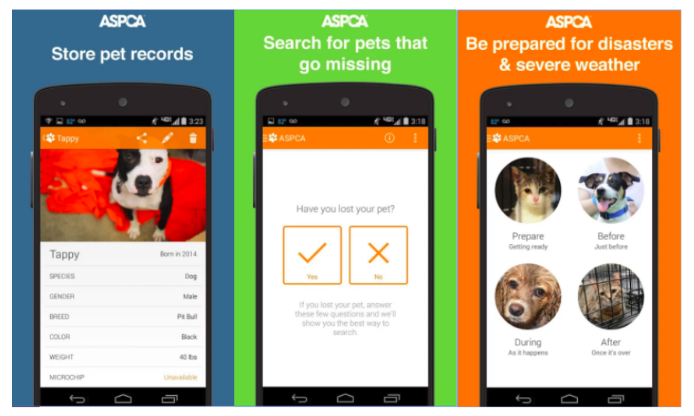
\includegraphics[width=1\textwidth]{Images/Ch1/ASPCA}
		\caption{ASPCA – Emergency Pet Safety}
		\label{fig:aspca}
	\end{figure}
	
	
	\underline{Fonctionnalités offertes}
	\begin{itemize}
		\item Déclarer la perte d’animal de compagnie.
		\item conseils pour prendre soin de l'animal.
		\item stocker un dossier médical de l’animal.
	\end{itemize} 
	\subsubsection{Dogalize} 
	Dogalize est une application destinée aux activistes animalier qui offre le partage de publication ou de statuts. Vous pourrez également obtenir de l'aide auprès des vétérinaires, discuter avec vos amis, demander des conseils à la communauté. Avec les cartes Dogalize, ou se trouve des activités et des endroits accueillants pour les animaux de compagnie\\
	
	\begin{figure}[H]
		\centering
		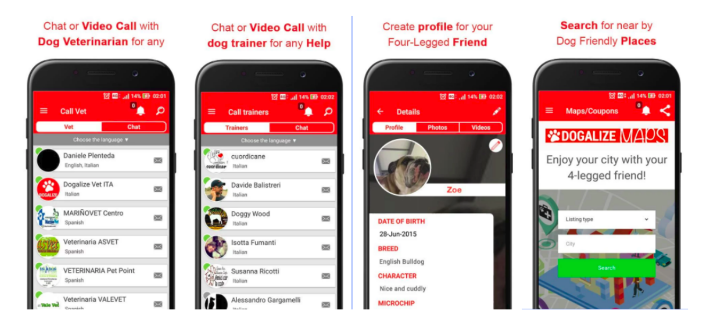
\includegraphics[width=1\textwidth]{Images/Ch1/Dogalize}
		\caption{Dogalize}
		\label{fig:dogalize}
	\end{figure}
	
	\underline{Fonctionnalités offertes}
	\begin{itemize}
		\item Partage de publication ou de statuts 
		\item Trouver des conseils.
		\item Échanger messages avec les autres utilisateurs.
		\item Obtenir l’aide des spécialistes tel que vétérinaire, dresseur, …
		\item Trouver des foyers d’animaux proches ou même des espaces d’activité.
	\end{itemize}
	\subsubsection{Pet First Aid - Red Cross}
	L'application de secourisme pour animaux de compagnie de la Croix-Rouge américaine met des conseils vétérinaires pour les urgences quotidiennes dans la paume de main. Avec des vidéos, des quiz interactifs et des conseils simples.\\
	\begin{figure}[H]
		\centering
		\includegraphics[width=1\textwidth]{"Images/Ch1/Pet first aid"}
		\caption{Pet First Aid - Red Cross}
		\label{fig:pet-first-aid}
	\end{figure}
	
	
	
	\underline{Fonctionnalités offertes}
	\begin{itemize}
		\item Obtenir l’aide des vétérinaires
		\item Consulter des conseils d’animalerie
		\item Localisez votre hôpital vétérinaire d'urgence ou animaux de compagnie hôtels les plus proches
		\item Personnaliser les profils d'animaux multiples et nominations vétérinaires établies.
	\end{itemize}
	\subsubsection{YummyPets}
	C’est une plateforme communautaire au service du propriétaire de l'animal de compagnie. Elle offre plusieurs service d’animalerie\\
	\begin{figure}[H]
		\centering
		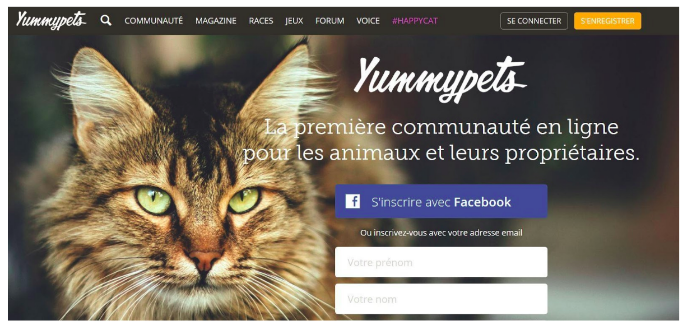
\includegraphics[width=1\textwidth]{Images/Ch1/Yummy-pet}
		\caption{Yummy Pets}
		\label{fig:yummy-pet}
	\end{figure}
	
	\underline{Fonctionnalités offertes}
	\begin{itemize}
		\item Permettre aux utilisateurs d’échanger des nouveautés
		\item Conseils pour prendre soin des animaux de compagnie
		\item Vente de produits d’animalerie
	\end{itemize}
	\subsection{Les solutions des réseaux sociaux}
	\begin{flushleft}
		Un réseau social est une structure formée par des relations entre des personnes. C’est un regroupement d’individus ou d’organisations qui discutent et interagissent entre eux. Ils partagent des opinions, des idées ou encore du contenu multimédia.
		Le plus connus et le plus utilisé des réseaux sociaux a present est Facebook 
		.
	\end{flushleft}
	
	\subsubsection{Facebook}
	\begin{figure}[H]
		\centering
		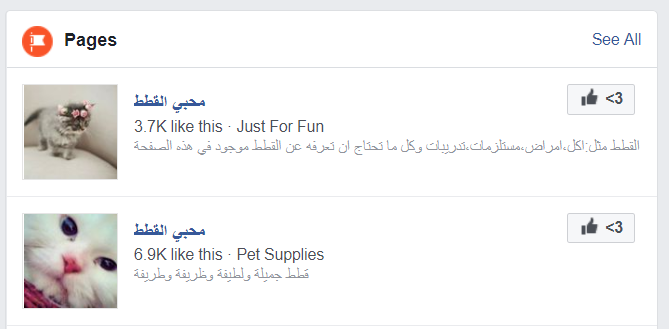
\includegraphics[width=1\linewidth]{Images/Ch1/1}
		\caption{Pages Facebook}
		\label{fig:1}
	\end{figure}

	\begin{figure}[H]
		\centering
		
\includegraphics[width=1\linewidth]{Images/Ch1/2}
		\caption{Groupes Facebook}
		\label{fig:2}
	\end{figure}
	Tant que Facebook permet aux utilisateurs de créer des pages , des groupes, des événements gratuitement, les activistes animalier ont appuyé sur ces fonctionnalités pour créer des communautés a travers Facebook , en créant des pages, des groupes et en lançant des événements  pour ceux qui s'intéressent aux bénévoles pour les animaux ainsi ils ont pu partager leurs intérêt envers les animaux et déclarer des états d’urgences pour obtenir de l’aide.\\ Pourtant cette solution reste manquante et incomplète pour couvrir les besoins des activistes animalier puisque Facebook est un réseau social grand public et n’est pas destiné pour ce genre d'activités.
	\subsection{Discussion}
	Les solutions existantes de plateforme d’intervention et de secourisme regroupent plusieurs fonctionnalités et chacune offre des fonctionnalités intéressantes mais un peu limités et parfois payantes. Mais une telle plateforme n’existe pas encore qui englobe la plupart des fonctionnalités et y ajoutes d’autres. Dans ce qui suit nous allons plus détailler les différences technique et fonctionnelle ainsi tirer les avantages et inconvénients de chaque solution.\\ \\
	Nous représentent ci-dessous une étude comparatif des critères techniques et fonctionnelles des applications connexes et solutions des réseaux sociaux \\
	\subsubsection{Comparaison technique}
	Pour effectuer une critique technique nous avons appuyer notre comparaison sur des critères qu'on trouve essentielle pour toutes application . Ci dessous , nous définissons chaque critère .  \\
	\underline{\textbf{Les critères Techniques:} }\\ \\
	\textbf{Ergonomie et graphisme:} Le même graphisme sur tous les OS.\\
	\textbf{Mise a jour du contenu:} Simple et immédiate.\\
	\textbf{Simplicité:} L'utilisation assez simple indépendamment du connaissance de l'utilisateur en informatique.\\
	\textbf{Exhaustivité:} L'application doit satisfaire les besoins des utilisateurs (La recherche, la demande, validation de qualité de service...).\\
	\textbf{Qualité de service:} Elle doit rendre ce service efficacement (de manière complète, pertinente, être toujours disponible, fiable, être pérenne et peu cher, facile et agréable à prendre en main et à utiliser...).\\
	\textbf{Accès conditionnées:} L'application doit garantir la confidentialité et la protection des données personnelles.\\
	\textbf{Rapidité:} Vitesse de traitement et de réponse aux évènements\\
	\textbf{Performance:} Capacité à réaliser et répondre rapidement aux demandes des utilisateurs.\\
	\textbf{Evolutivité/Agilité:} Capacité à évoluer vite et sur spécifications changeantes.
	\begin{figure}[H]
		\centering
		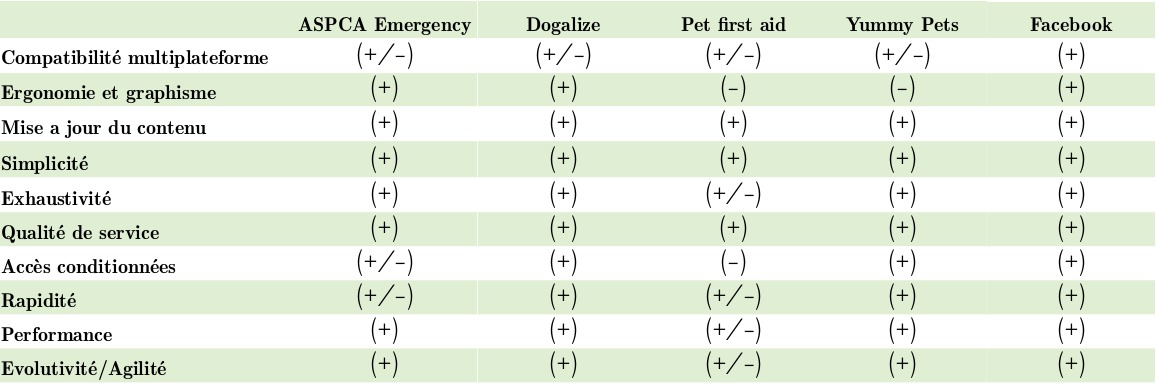
\includegraphics[width=1.3\textwidth]{Images/Ch1/technique}
		\caption{Comparaison technique entre les solutions existantes}
		\label{fig:comparaison-technique}
	\end{figure}
	\vspace*{\fill}
	
	\subsubsection{Comparaison technique}
	\underline{\textbf{Critères fonctionnelle:}}
	
	\begin{figure}[H]
		\centering
		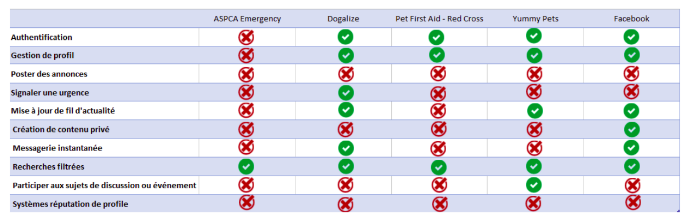
\includegraphics[width=1.3\textwidth]{Images/Ch1/comparaison-fonctionnelles}
		\caption{Comparaison fonctionnelles entre les solutions existantes}
		\label{fig:comparaison-fonctionnelles}
	\end{figure}
	
	
	
	\section{Solution proposée }
	Suite à la définition des réseaux sociaux et d'après les avantages qu’offre un réseau social, notre solution consiste en une plateforme sous forme d’un réseau sociale permettant de venir en aide à des animaux perdus, errants ou à donner.Cette plateforme est dédié aux personnes qui défendent les animaux et leur droits appelés aussi Pet Lovers ainsi que les communautés et groupes qui apportent le plus dans le domaine de secourisme d’animaux.
	
	Notre solution offre une partie public front-office accessible par tous utilisateurs et une partie privé à l’administration back-office accessible pour les administrateurs qui permet le contrôle .
	
	Dans la figure ci dessous nous essayerons de résumer les principaux fonctionnalités  de notre solution .
	\\
	\begin{figure}[H]
		\centering
		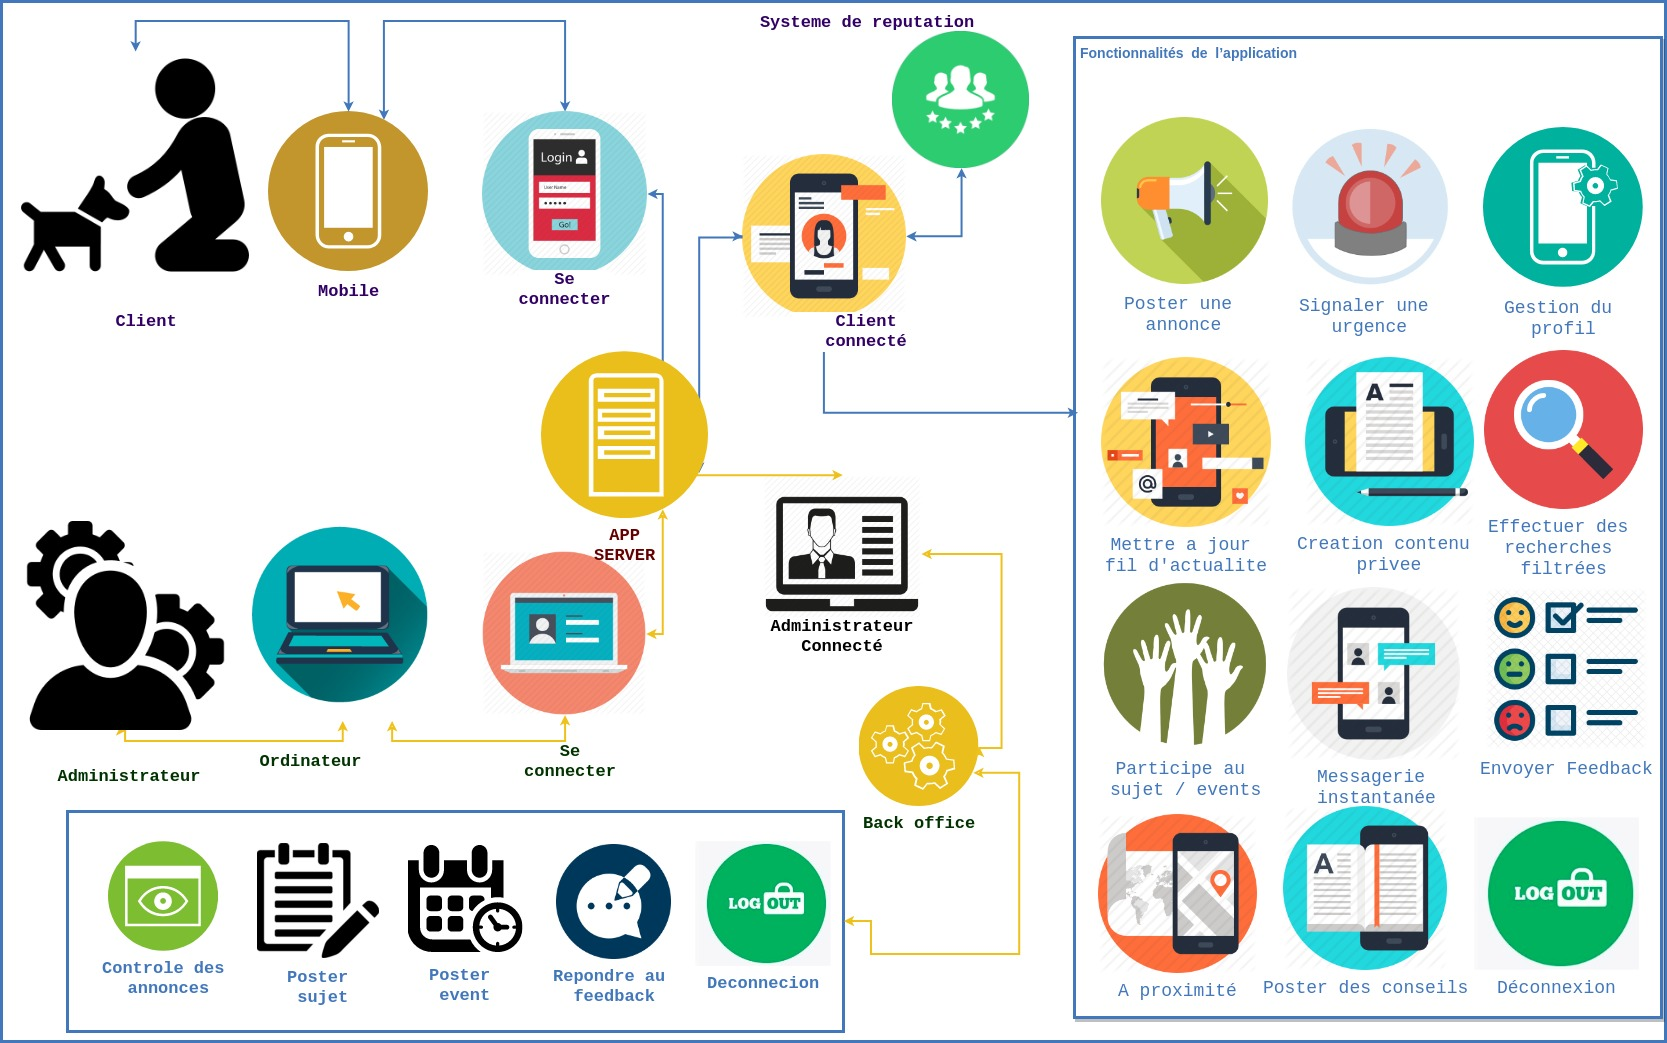
\includegraphics[width=1.3\textwidth]{Images/Ch1/objectives}
		\caption{Description des principaux fonctionnalités}
		\label{fig:objectives}
	\end{figure}
	
	
	\section{Méthodologie de réalisation }
	Une méthodologie de développement est un cadre utilisé pour structurer, planifier et contrôler le développement d’une application. Suivre une méthodologie de développement permet de baser un projet sur un modèle de conception et des formalismes de notations ce qui implique la réduction des coût de développement et encourager la communication entre les personnes . Il existe une diversité de méthodologies disponibles et chacune offre des avantages donc choisir une n’est pas une tache facile . Pour ca nous procéderons a une etude a propos les methodes existantes pour degager la methodologie la plus adéquate a notre equipe et a notre projet .
	
	\subsection{Modèle en V}
	Le cycle en V est un paradigme du développement informatique. Il décrit les étapes essentielles
	du développement d’un logiciel, le cycle de vie du projet. Il est représenté par un V dont la branche
	descendante contient toutes les étapes de la conception du projet, et la branche montante toutes les étapes de tests du projet. La pointe du V, quant à elle, représente la réalisation concrète du projet,
	le codage ; on pourrait donc en déduire, de manière simpliste, que les deux branches montantes et
	descendantes ne sont que de la documentation.\\
	\underline{\textbf{Avantages :}}
	\begin{itemize}
		\item Meilleure validation intermédiaire(Bon suivi de projet, favorise la décomposition fonctionnelle de l’activité).
		\item Modèle éprouvé très utilisé pour de grands projets.
		\item  Facile de prévoir les tests à réaliser au moment ou l’on conçoit une fonctionnalité ou une
		interface.
		\item Permet d’espérer que le livrable final sera parfait, puisque les étapes de test sont aussi nombreuses que les étapes de réflexion.
		\item Il est facile de prévoir les tests à réaliser au moment où l’on conçoit une fonctionnalité ou
		une interface.
		\item Le travail s’enchaîne de façon assez naturelle.
	\end{itemize}
	\underline{\textbf{Inconvenients :}}
	\begin{itemize}
		\item Rarement utilisé tel quel et le V est bien souvent déséquilibré .
		\item Un modèle toujours séquentiel.
		\item Adapté aux problèmes bien connus c’est à dire il est idéal quand les besoins sont bien connus, quand l’analyse et la conception sont claires.
		\item Le manque de souplesse : chaque phase doit être terminée (spécification, conception, développement) avant de passer à la suivante. Chacune des étapes va durer plus longtemps et donc coûter plus chère.
		\item La péremption du produit : sur de gros projets dont la durée de réalisation est de plusieurs années.
	\end{itemize}
	
	\subsection{Modèle en Scrum}
	Scrum est aujourd’hui la méthode agile populaire. Elle se caractérise par itérations assez courts et un formalisme réduit.
	Le cycle de vie dans un projet SCRUM est composé de :
	Phase d’initialisation :Phase linéaire aux processus explicitement connus et dont les inputs
	et les outputs sont bien déterminés.
	Phase de cloture : est aussi une phase linéaire dont le processus sont clairement définis.\\
	\underline{\textbf{Avantages :}}
	\begin{itemize}
		\item Personnel engagé : l’une des caractéristiques de SCRUM, c’est que le personnel participe
		activement à la définition des activités et des horaires, de sorte que le degré d’engagement
		et la motivation sont plus élevé.
		\item Simplicité des processus.
		\item Augmentation de productivité.
		\item Amélioration de la communication.
		\item Flexibilité de changement.
		\item Simplicité, efficacité et qualité.
		\item Esprit d’équipe.
	\end{itemize}
	\underline{\textbf{Inconvenients :}}
	\begin{itemize}
		\item Violation de responsabilité.
		\item Cette méthodologie a besoin de membres expérimentés de l’équipe seulement. si l’équipe se compose de personnes qui sont novices, le projet ne peut pas être achevé à temps.
		\item Faible documentation et donc facile à détourner.
	\end{itemize}
	\subsection{Modèle RUP}
	Rational Unified Process, instanciation par Rational Software (IBM) des préceptes UP(processus unifié). Le principe de cette méthode est de parcourir un cycle de vie durant une itération. Chaque phase du cycle de vie est très précisément détaillé. C’est une méthode générique, itérative et incrémentale. Il divise le processus de développement en quatre phases :
	Inception :L'idée de ce projet est déclarée. L’équipe de développement détermine si le projet
	mérite d'être poursuivi et quelles ressources seront nécessaires.
	Elaboration : L’architecture du projet et les ressources nécessaires sont encore évalués .
	Les développeurs considèrent les applications possibles du logiciel et les associés au développement.
	Construction : Le projet est développé est complété. Le logiciel est conçu, écrit et testé.
	Transition : Le logiciel est diffusé au public. Les derniers ajustements ou mise à jour sont effectués en fonction des commentaires finaux des utilisateurs.\\
	\underline{\textbf{Avantages :}}
	\begin{itemize}
		\item RUP est l’une des plus célèbres implémentations de la méthode PU permettant de donner un cadre au développement logiciel.
		\item Le RUP est plus documenté et donc peut être plus guidé.
		\item Traçabilité à partir des Uses Cases jusqu’au déploiement.
		\item Approche basé sur l’architecture.
		\item Gestion des risques dans les projets.
		\item Cadre propice à la réutilisation
		\item Moins couteux de changer la portée
		\item Certaines fonctionnalités de travail peut être développé rapidement et tot dans le cycle de vie.
	\end{itemize}
	\underline{\textbf{Inconvenients :}}
	\begin{itemize}
		\item Coût de personnalisation souvent élevé.
		\item Plus de ressources peuvent être nécessaires.
		\item Chaque phase d’une itération est rigide sans chevauchements.
		\item Plus de ressources peuvent être nécessaires.
		\item Vision non évidente.
		\item Processus très axé.
	\end{itemize}
	
	\subsection{Modèle en 2TUP}
	La méthode 2TUP préconise un cycle de vie en Y qui dissocie et parallélisé la résolution des
	questions fonctionnelles et techniques. Le cycle de vie de 2TUP s’apparente à un cycle en cascade mais introduit une forme itérative interne à certaines tâches.\\
	\underline{\textbf{Avantages :}}
	\begin{itemize}
		\item Modèle d’analyse réutilisable.
		\item Itératif.
		\item Indépendant de la taille du projet.
		\item Prise en compte de la gestion et du technologique.
		\item Ne définis pas le typlogies d’intervenants et les livrables.
	\end{itemize}
	\underline{\textbf{Inconvenients :}}
	\begin{itemize}
		\item Il y a un manque d’accent sur la conception et la documentation nécessaires.
		\item Couvre seulement la partie développement.
		\item Pas de documents types.
	\end{itemize}
	\textbf{Synthèse de méthodologie}
	Après cette comparaison, nous constatons que la méthodologie 2TUP est la plus efficace pour réaliser les différentes étapes de développement de notre application.
	\subsection{Mise en pratique du processus 2TUP }
	Le 2TUP propose un cycle de développement en Y, qui dissocie les aspects techniques des aspects fonctionnels. Le cycle de vie de 2TUP s’apparente à un cycle en cascade, mais introduit une forme itérative interne à certaines tâches .
	Nous avons choisi ce procesus vue son approche nouvelle, originale et surtout son adaptation au solutions des réseaux sociaux .
	Le processus 2TUP se résume clairement dans la figure suivante : 
	
	\begin{figure}[h]
		\centering
		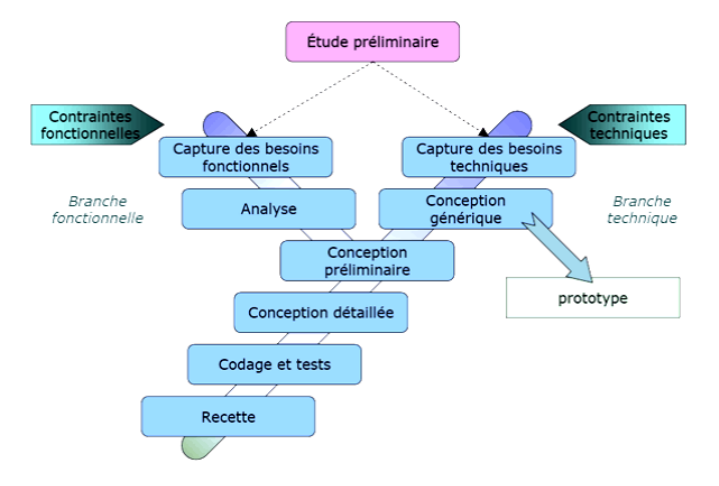
\includegraphics[width=1\textwidth]{Images/Ch1/2tup}
		\caption{Description du processus 2tup}
		\label{fig:2tup}
	\end{figure}
	
	
	Le processus 2TUP signifie que le processus suit deux chemin . Il s’agit du «chemin fonctionnels » et du « «chemin technique », qui correspondent aux deux axes de changement imposés au système d’information.
	\begin{enumerate}
		\item Branche fonctionnelle ou « gauche »
		Elle vise la capture des besoins fonctionnels et l'analyse des spécifications fonctionnelles de manière à déterminer ce que va réaliser le système en terme de métier. C'est ici, qu'on identifie et dégage toutes les fonctionnalités du système à réaliser.
		\item Branche technique ou « droite »
		Elle permet la capture des besoins non fonctionnels. Il s'agit essentiellement des contraintes que l'application doit prendre en compte comme par exemple les contraintes d'intégration, les contraintes de développement et les contraintes de performances.
		\item Branche du milieu ou phase de réalisation 
		A l’issue des évolutions du modèle fonctionnel et de l’architecture technique, la réalisation du système consiste à fusionner les résultats des 2 branches. Cette fusion conduit à l’obtention d’un processus en forme de Y.
	\end{enumerate}
	La méthodologie 2TUP se base sur le processus UP qui est de type adaptatif il est de plus :
	\begin{itemize}
		\item \textbf{Itératif et incrémental:}
		Le projet est découpé en des itérations de courte durée. Ces itérations aident à mieux suivre l'avancement du système global. A chaque itération, il est produit un exécutable de façon incrémentale.
		\item \textbf{Piloté par les risques:}  Il est identifié et écarté au plutôt tout risque pouvant conduire à un échec du projet. Le pilotage par les risques c’est :
		\begin{itemize}
			\item Analyser les risques potentiels au plus tôt
			\item Hiérarchiser les risques
			\item Associer un ensemble des cas d'utilisation à chaque risque
			\item Déclencher les itérations selon la criticité des uses cases qu’elles regroupent 
			\item UP propose une gestion des risques. Ce qui constitue une avancée significative.
		\end{itemize}
		\item\textbf{Piloté par les uses cases:}
		Pour servir les attentes des utilisateurs, on centre le processus de développement sur leurs besoins. On fait apparaître ces besoins à l’aide de la technique des cas d’utilisation : à l’aide d’une capture des besoins fonctionnels d’un système et en orientant le travail de chaque itération. Ils vont guider le processus à travers l’utilisation des différents modèles UML qui représentent le système.
		\item\textbf{Centré sur l'architecture:}
		Le système est décomposé en modules pour des besoins de maintenabilité et d'évolutivité.
		L’architecture doit prévoir la réalisation de tous les uses case et doit évoluer avec eux. Elle le fait en tenant compte de facteurs tels que :
		\begin{itemize}
			\item La plateforme d’exécution : matériel, système, BD, réseau, etc.
			\item Les composants réutilisables : librairies, caisses à outils, composants du commerce, etc.
			\item Les considérations de déploiement et les besoins non-fonctionnels : la performance, la fiabilité, la robustesse, etc.
		\end{itemize}
		\item\textbf{Conduit par les cas d'utilisation :} Le processus met en avant les besoins et exigences des futurs utilisateurs du système.
	\end{itemize}
\section{Diagramme de Gantt}
Le diagramme de Gantt, couramment utilisé en gestion de projet, est l'un des outils les plus efficaces pour représenter visuellement l'état d'avancement des différentes activités (tâches) qui constituent un projet. La colonne de gauche du diagramme énumère toutes les tâches à effectuer, tandis que la ligne d'en-tête représente les unités de temps les plus adaptées au projet (jours, semaines, mois etc.).\\
 Chaque tâche est matérialisée par une barre horizontale, dont la position et la longueur représentent la date de début, la durée et la date de fin. Ce diagramme permet donc de visualiser d'un seul coup d'œil toutes les tâches à accomplir pour mener le projet à bien, et indique la date à laquelle ces tâches doivent être effectuées (le planning).\\

\begin{itemize}
	\item Les différentes tâches à envisager
	\item La date de début et la date de fin de chaque tâche
	\item La durée escomptée de chaque tâche
	\item  La date de début et la date de fin du projet dans son ensemble
\end{itemize}
\begin{figure}[H]
	\centering
	\includegraphics[width=0.7\linewidth]{"Images/diagram de gantt"}
	\caption{Description du planning de travail ~ Diagramme de Gantt}
	\label{fig:diagram-de-gantt}
\end{figure}

	\section{Conclusion}
	Dans ce chapitre nous avons abordé la problématique présente puis on a procéder a l'étude de l'existant qui nous a permit de dégager les défauts technique et fonctionnelle des solutions présentes .\\
	En suite nous avons présenté notre solutions ainsi que les objectives qu'on vise atteindre .\\
	Enfin nous avons étudié les méthodologies de développement possible pour aboutir à la méthode 2TUP qu’on a bien expliquer avec une analyse détaillée.
	
	%%%%%%%%%%%%%%%%%%%%%%%%%%%%%%%%%%%%%%%%%%%%%%%%%%%%%%%%%%%%%%%%%%
	%                       CHAPITRE 2%                              %
	%%%%%%%%%%%%%%%%%%%%%%%%%%%%%%%%%%%%%%%%%%%%%%%%%%%%%%%%%%%%%%%%%%
	
	\chapter{Capture et spécification des besoins}
	\section{Introduction}	
	Dans ce chapitre, nous présentons les objectifs de notre application, ce qui nous amène à identifier les fonctionnalités du système en recensant les besoins fonctionnels, de connaître la liste des contraintes et exigences traduite par les besoins non fonctionnels et les besoins techniques qu’on va utiliser pour répondre aux fonctionnalités de notre projet.
	La spécification des besoins doit décrire sans ambiguïté l’application à développer et toutes les personnes impliquées dans le projet doivent avoir accès à la spécification des besoins.
	
	\section{Capture des besoins}
	Dans cette partie nous allons détailler nos besoins qui se divisent en 3 types : besoins fonctionnels, besoins non fonctionnels et enfin les besoins techniques.
	\subsection{Capture des besoins fonctionnels}
	Notre application offre une partie public appelé front-office accessible par tous utilisateurs et une partie privé à l’administration appelé back-office accessible pour les administrateurs pour permettre les tâches de contrôles et chaque partie offre des fonctionnalités distinctes de l’autre 	
	\subsubsection{Front-Office}
	\textbf{Authentification:}  Permettre aux utilisateurs de créer leurs comptes pour se connecter avec leur adresse mail et mot de passe ou s’authentifier via leur compte des réseaux sociaux ( Facebook , Gmail ).\\
	\textbf{Compléter les informations} du profil en ajoutant des informations secondaires.\\
	\textbf{Poster des annonces à propos d’un animal selon ses conditions :}
	\begin{itemize}
		\item \textbf{Besoin d’aide (A3):} L’animal a besoin d’aide d’une personne à proximité.
		\begin{itemize}
			\item La notification de ces annonces atteints les utilisateurs dans une zone géographique limitée à 2 Km .
		\end{itemize}
		\item \textbf{Besoin d’un foyer (A2):} L’animal a besoin d’un foyer d'accueil .
		\begin{itemize}
			\item La notification de ces annonces atteints les utilisateurs dans une zone géographique limitée à 4 Km .
		\end{itemize}
		\item \textbf{Besoin d’un spécialiste (A1):} L’animal est blessé , malade et une 
		intervention d’un spécialiste est nécessaire
		\begin{itemize}
			\item La notification de ces annonces atteints les utilisateurs dans une zone géographique limitée à 8 Km 
		\end{itemize}
		\item \textbf{Animal en danger (A0):} l’animal est en danger et une intervention 
		immédiate est nécessaire 
		\begin{itemize}
			\item La notification de ces annonces atteints les utilisateurs dans une zone géographique limitée à 10 Km .
		\end{itemize}
	\end{itemize}
	
	\textbf{NB:} Pour poster une annonce de type A1 ou A0 l’utilisateur doit disposer d’au moin 30 points de réputation.\\
	
	\textbf{Signaler une urgence : } le signale d’urgence se fait lorsqu’un utilisateurs poste une annonce de type A1 ou A0 . ainsi ce type d’annonce serait visible en premier et la notification atteindra les utilisateurs dans une zone géographique plus large que les autres types d’annonces (A2 , A3).\\
	
	\textbf{Gérer le profil :} chaque utilisateur aura un profil consultable ou il peut ajouter des conseils et des publications.
	Il peut aussi accéder aux paramètre pour changer ses informations du profil et du compte.\\
	
	\textbf{Consulter fil d'accueil :} 
	Un utilisateur peut visualiser les publications partagé par ses amis, les commenter,les aimer et sauvegarder des conseils.\\
	
	\textbf{Gestion du contenu privé :} Visualise les conseils sauvegardé récemment  \\
	
	\textbf{Messagerie instantanée :} l’application permet l'échange de messages instantanées entre les utilisateurs.\\
	
	\textbf{Envoyer des feedbacks :} 
	Les utilisateurs peuvent envoyer des feedback aux administrateur pour suggérer des idées ,  porter plaintes , donner son avis.\\
	
	\textbf{Participer aux sujets de discussions :} Les administrateurs de l’application peuvent publier des sujet de discussion en relation avec des événements internationaux a propos des animaux où les utilisateurs pourront participer à ces sujets en commentant leurs avis , des solutions , échanger des idées.\\
	
	\textbf{Systèmes de réputation de profil :} Le système de réputation de profil est un système qui permet à l’utilisateur d'évoluer son profil en augmentant ses points de réputation ce qui lui permet plus de privilèges.\\
	
	Dans notre application , initialement l’utilisateur commence par une réputation égale à 1 , puis à chaque action effectué il augmente ses point de réputation : 
	\begin{itemize}
		\item Completer toute les informations du profil : +5 pts
		\item Publier des conseils : +3pts
		\item Poster des annonces 
		\begin{itemize}
			\item Type A3 : +4pts
			\item Type A2 : +6pts 
			\item Type A1 : +10pts 
			\item Type A0 : +12pts
			\item Autre : +1pts
		\end{itemize}
		\item Commenter / Aimer une annonce + 2pts
		\begin{itemize}
			\item Propriétaire de l’annonce : +2pts
		\end{itemize}
		\item Partager une annonce : +4pt
		\begin{itemize}
			\item Propriétaire de l’annonce : +4pts
		\end{itemize}
		\item Participation au sujet de discussion :
		\begin{itemize}
			\item Commenter : +2pts
			\item Partager le sujet : +3pts
		\end{itemize}
	\end{itemize}
	\subsubsection{Back-Office}
	\textbf{S’authentifier :} L’administrateur peut s’identifier avec son adresse mail et un mot de passe\\
	\textbf{Contrôle des annonces :}
	\begin{itemize}
		\item Majorer ou minorer l'état d’urgence d’une annonce .
		\item Supprimer une annonce
	\end{itemize}
	\textbf{Gérer des sujet de discussion :} L’administrateur peut poster un sujet de discussion . Ce poste sera visible à tous les utilisateurs . il peut aussi modifier ou supprimer un sujet .\\
	\textbf{Répondre au feedback :} L’administrateur peut consulter les messages envoyé par les utilisateurs ( feedback , plainte , avis , … ) et répondre .
	\subsection{Capture des besoins non-fonctionnels}
	Les besoins non-fonctionnels représente les points qui agissent sur la satisfaction et le rendement de l’utilisateur de façons indirectes .
	notre application doit être à la mesure des points suivants : \\
	\textbf{Ergonomie et graphisme :}  Le même graphisme sur tous les OS.\\
	\textbf{Mise à jour du contenu :} Simple et immédiate.\\
	\textbf{Simplicité :} L’utilisation assez simple indépendamment de la connaissance de l’utilisateur en informatique.\\
	\textbf{Performance :} Capacité à réaliser et répondre rapidement aux demandes
	des utilisateurs.\\
	\textbf{Accès conditionnées :} L’application doit garantir la confidentialité et la protection des données personnelles.\\
	\textbf{Rapidité :} Vitesse de traitement et de réponse.
	\subsection{Capture des besoins techniques}
	Technologie les plus utilisé pour le développement des applications mobile :
	
	\begin{center}
		\begin{tabular}{ |p{2cm}|p{1.5cm}|p{5.5cm}|p{5.5cm}|  }
			\hline
			{\centering 
				Technologie}
			& 
			{\centering 
				Langage
			} & 
			{\centering 
				Avantages
			} & 
			{\centering 
				Inconvenients
			} 
			\\ 
			\hline
			\vspace*{\fill}
			{\centering Android\par} &
			\vspace*{\fill} Java / Kotlin &
			\vspace*{\fill}
			\begin{itemize}
				\item Langage de programmation facile à maîtriser 
				\item Plateforme de développement ouverte
				\item Environnement de développement complet
			\end{itemize} 
			
			&  \vspace*{\fill}
			\begin{itemize}
				\item N’est pas multiplateforme
				\item Le développement d’une application prend plus du temps par rapport aux autre plateformes
				\item Environnement puissant nécessitant l’utilisation d’un matériel puissant
			\end{itemize}
			
			
			\\ 
			\hline
			\vspace*{\fill}
			
			{\centering IOS \par} & \vspace*{\fill} Objective-C/Swift &
			\vspace*{\fill}
			\begin{itemize}
				\item Environnement de développement complet
				\item Securité garantie
			\end{itemize}
			&  \vspace*{\fill}
			\begin{itemize}
				\item Langage de programmation pas trop répandue comme java
				\item Plus coûteux que les autre plateforme
			\end{itemize}
			\\ 
			\hline
			\vspace*{\fill}
			{\centering Ionic  \par}& 
			\vspace*{\fill} Html + Css  + TypeScript & 
			\vspace*{\fill} \begin{itemize}
				\item Langage de programmation facile et maîtrisable , le même du développement web
				\item Multiplateforme , un seul code executable sur ios et android
				\item Disponibilé des plugins
				\item Composant prêt à l’utilisation .
			\end{itemize}
			& \vspace*{\fill}
			\begin{itemize}
				\item Ne supporte pas le développement des applications 3D
				\item Necessite une connaissance du framework Angular
			\end{itemize} 
			
			\\ 
			\hline
		\end{tabular}
	\end{center}
	Technologie les plus utilisé pour le développement des applications web :
	
	\begin{center}
		\begin{tabular}{ |p{2cm}|p{4cm}|p{4.4cm}|p{4.4cm}|  }
			\hline
			\vspace*{\fill}
			{\centering 
				Technologie\par
			}
			& \vspace*{\fill} {\centering
				Description\par
			} & \vspace*{\fill} {\centering
				Avantages\par
			}  & \vspace*{\fill} {\centering
				Inconvenients\par
			}\\ 
			\hline
			\vspace*{\fill}
			PHP (Back End) & \vspace*{\fill} C’est un langage interprété exé-
			cuté du côté serveur et non du
			côté client. La syntaxe de lan-
			gage provient de celles du lan-
			gage C, du Perl, du java. La pos-
			sibilité d’inclure le script PHP au
			sein d’une page HTML.
			& \vspace*{\fill} 
			\begin{itemize}
				\item Il est gratuit.
				\item Il ne nécessite pas
				beaucoup de code
				pour obtenir un ré-
				sultat.
				
				\item L’hébergement du
				PHP est supporté
				presque partout.
				
				\item Aucun typage des
				variables.
				
			\end{itemize}
			&  \vspace*{\fill}
			\begin{itemize}
				\item Manque de vision
				pour le dévelop-
				pement de gros
				projet.
				
				\item Beaucoup de failles
				de sécurité
			\end{itemize}
			\\ 
			\hline
			\vspace*{\fill}
			Angular (Front End) & \vspace*{\fill}
			C’est une framework de développement d’application web coté client ( front End) en utilisant le langage typescript en plus du html et css
			& \vspace*{\fill}
			\begin{itemize}
				\item Amélioration de la réactivité de l’interface de l’utilisateur 
				\item Ouvert 
				\item Grande communauté et très utilisés
				\item Langage de programmation simple
			\end{itemize}
			& \vspace*{\fill} -architecture de l’application un peu complexe\\ 
			\hline
			
		\end{tabular}
	\end{center}
	
	\section{Technologies utilisées }
	Les technologies que nous allons utiliser sont les suivantes : 
	\begin{itemize}
		\item Firebase comme un système de back end de gestion et de manipulation de données .
		\item Le Framework ionic 3 coté front end de l’application mobile .
		\item Le Framework Angular 5 coté front end du site web du back office .
	\end{itemize}
	\section{Spécification des besoins fonctionnels }	
	\subsection{UML}
	UML (Unified Modeling Language) est une méthode de modélisation orientée objet développée en réponse à l’appel à propositions lancé par l’OMG (Object Management Group) dans le but de définir la notation standard pour la modélisation des applications construites à l’aide d’objets.
	C’est est une méthode utilisant une représentation graphique. L’usage d’une représentation graphique est un complément excellent à celui de représentations textuelles. 
	En effet, l’une comme l’autre sont ambiguës mais leur utilisation simultanée permet de diminuer les ambiguïtés de chacune d’elle. Il est couramment utilisé en développement logiciel et en conception orienté objet
	
	\subsection{Diagramme de cas d’utilisation}
	Le diagramme de cas d’utilisation décrit les principales fonctionnalités du système offertes aux acteurs .\\
	Dans notre application nous avons 3 types d’acteurs : 
	
	\begin{itemize}
		\item \underline{Invité:} cet acteur est invité à créer un compte ou se connecter pour pouvoir accéder à l’ensemble des services de l’application 
		\item \underline{Utilisateur:}  C’est l’acteur principal , il possède un compte et peut exploiter les fonctionnalité du front office cité ci dessus via l’application mobile.
		\item  \underline{Administrateur:} il possède un compte privé qui lui permet d’exploiter les fonctionnalités du back office via le site web .
	\end{itemize}
	\subsubsection{Diagramme de cas d’utilisation global}
	La figure ci-dessous représente le diagramme de cas d’utilisation global qui donne une vue générale de comportement fonctionnel de notre application mobile/web. Elle représente les acteurs en interaction avec le système ainsi que ces différentes fonctionnalités.
	
	\begin{figure}[H]
		\centering
		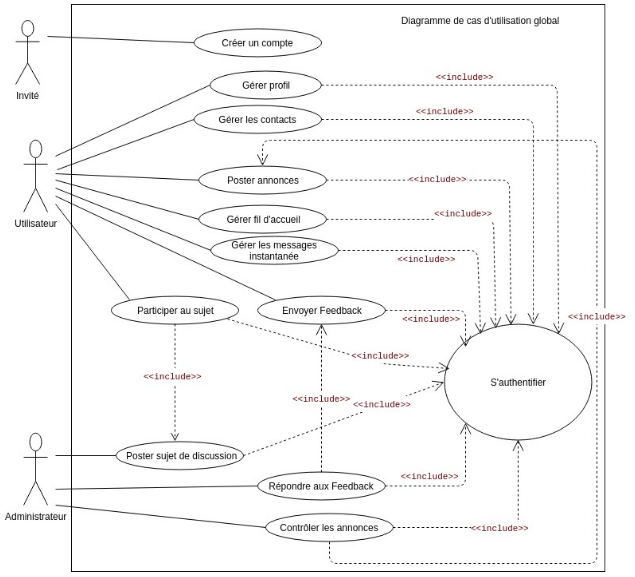
\includegraphics[width=16cm, height=17cm]{Diagrammes/Cas_global}
		\caption{Diagramme de cas d’utilisation global}
		\label{fig:casglobal}
	\end{figure}
	
	\subsubsection{Cas d’utilisation : Gérer profil}
	\begin{figure}[H]
		\centering
		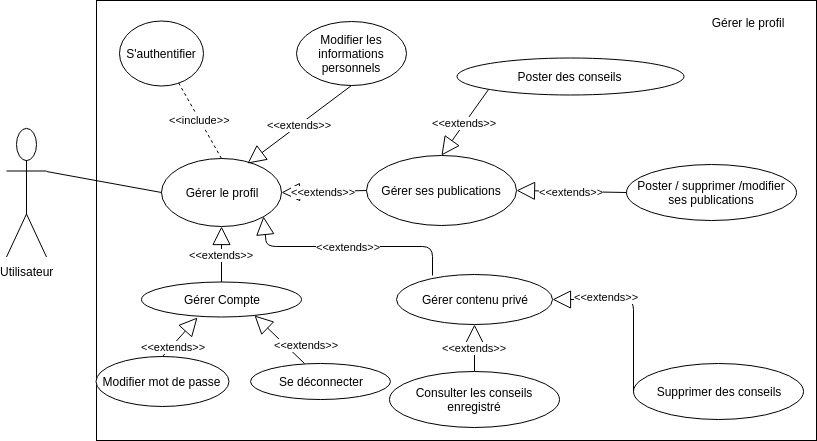
\includegraphics[width=1\textwidth]{Diagrammes/gerer_profil}
		\caption{Diagramme de cas d’utilisation « Gérer profil »}
		\label{fig:gererprofil}
	\end{figure}
	
	\begin{tabular}{ |p{3cm}|p{8cm}|  }
		
		\hline
		Titre& Gérer le profil \\
		\hline
		Description  & L’utilisateur a la possibilité de gérer son profil\\
		\hline
		Acteur&Utilisateur .\\
		\hline
		Pré-Condition &S’authentifier.
		\\
		\hline
		\multicolumn{2}{|c|}{Scénario normal} \\
		\hline
		1- Modifier ses informations personnelles & L’utilisateur peut modifier ses informations personnel tel que numéro de téléphone , langue , adresse ou description .\\
		
		2- Gérer ses publication & 
		\begin{itemize} 
			\item Créer conseil 
			\item Gérer contenu privée
			\item Gérer des publications normales 
			\end {itemize} \\
			3- Gérer Compte&
			\begin{itemize}
				\item Modifier mot de passe 
				\item Se déconnecter
			\end{itemize}\\
			\hline
			Post-Condition& Profil géré\\
			\hline
			Exception&  Pas d’accès internet .\\
			\hline
		\end{tabular}
		
		\subsubsection{Cas d’utilisation : Gérer les contacts }
		
		\begin{figure}[H]
			\centering
			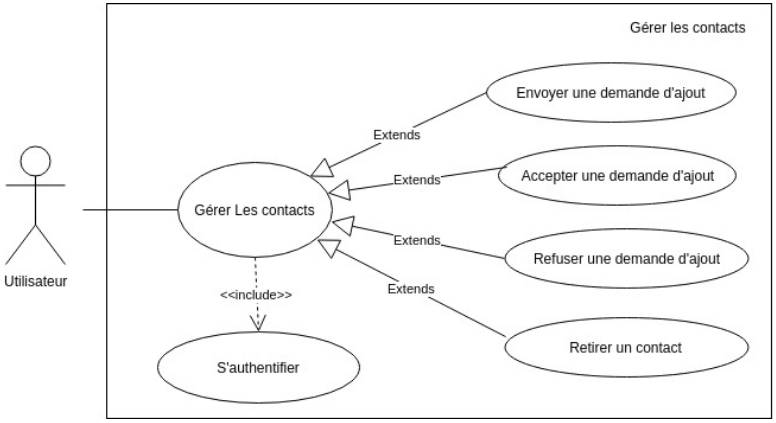
\includegraphics[width=1\textwidth]{Diagrammes/gerer_contact}
			\caption{Diagramme de cas d’utilisation « Gérer les contacts »}
			\label{fig:gerercontact}
		\end{figure}
		
		\begin{tabular}{ |p{4cm}|p{9cm}|  }
			
			\hline
			Titre&  Gérer les contacts\\
			\hline
			Description  & L’utilisateur a la possibilité de gérer ses contacts\\
			\hline
			Acteur& Utilisateur\\
			\hline
			Pré-Condition & S’authentifier.
			\\
			\hline
			\multicolumn{2}{|c|}{Scenario normal} \\
			\hline
			
			1.Envoyer une demande d’ajout : & \begin{itemize}
				\item L’utilisateur sélectionne le contact et lui envoi une invitation .
			\end{itemize}\\
			2.Accepter une demande d’ajout : & \begin{itemize}
				\item Le système notifie l’utilisateur qu’il a une nouvelle demande d’ajout.
				\item L’utilisateur consulte sa liste d’invitation et accepte/refuse la demande d’ajout.
			\end{itemize}\\
			3.Retirer un contact : & \begin{itemize}
				\item L’utilisateur consulte la liste de ses contacts.
				\item Il sélectionne le contact à retirer.
			\end{itemize}\\
			
			
			
			% \multicolumn{2}{|c|}{2-} \\
			% \multicolumn{2}{|c|}{3- } \\
			% \multicolumn{2}{|c|}{4- } \\
			
			\hline
			Post-Condition&Liste de contact géré \\
			\hline
			Exception& Pas d’accès internet .\\
			\hline
		\end{tabular}
		\subsubsection{Cas d’utilisation : Poster des annonces}
		\begin{figure}[H]
			\centering
			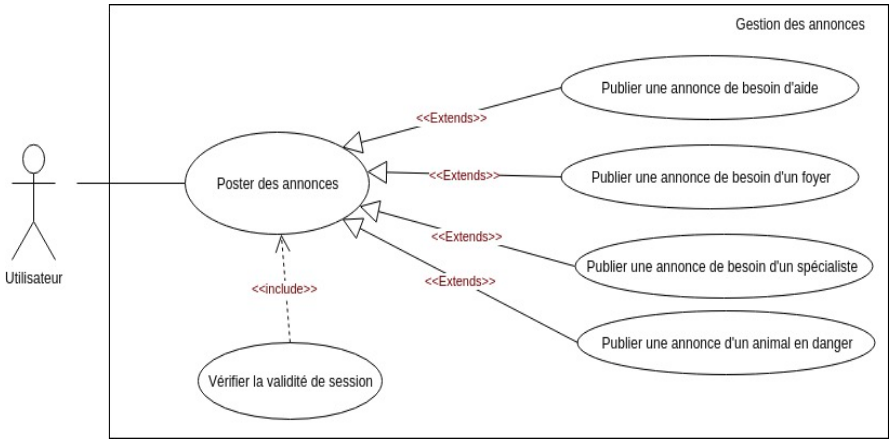
\includegraphics[width=1\textwidth]{Diagrammes/poster_annonces}
			\caption{Diagramme de cas d’utilisation « Poster des annonces »}
			\label{fig:posterannonces}
		\end{figure}
		
		\begin{tabular}{ |p{3cm}|p{11cm}|  }
			
			\hline
			Titre&  Poster des annonces\\
			\hline
			Description  &L’application permet aux utilisateurs de publier des annonces d’animaux en cas d’urgences de 4 types (annonce de besoin d’aide A3, annonce de besoin de
			foyer A2, annonce de besoin d’un spécialiste A1, annonce d’un animal en danger A0).
			\\
			\hline
			Acteur&Utilisateur\\
			\hline
			Pré-Condition &Vérification de la validité de session et la réputation de l’utilisateur en cas d’une annonce du type A1 ou A0 et l’activation du GPS 
			\\
			\hline
			\multicolumn{2}{|c|}{Scenario normal} \\
			\hline
			Déclarer une annonce& 	L’utilisateur doit choisir le type d'annonce, puis accéder à l’interface de déclaration d’annonce où il doit introduire une description et il peut aussi ajouter des images et il précise sa localisation.
			
			
			\vspace{5mm} %5mm vertical space
			Dans le cas ou la réputation de l’utilisateur est supérieure à 30 points , il peut poster une annonce de n’importe quel type.
			
			
			\vspace{5mm} %5mm vertical space
			Dans le cas ou la réputation de l’utilisateur est inférieur à 30 points , il a le droit de poster des annonces seulement de type A3 ou A2 .
			
			
			\vspace{5mm} %5mm vertical space
			L’avantage des annonces A0 et A1 est que la notification de ces annonces atteints les utilisateurs dans une zone géographique de 8 Km pour A1 et 10 Km pour A0 .
			\\
			
			\hline
			Post-Condition& Annonce publiée\\
			\hline
			Exception&  • Exception 1 :Champs obligatoires incomplets 
			
			• Exception 2 : Désactivation du GPS
			
			
			• Exception 3 : Pas d'accès Internet .\\
			\hline
		\end{tabular}
		\subsubsection{Cas d’utilisation : Gérer fil d'accueil }
		\begin{figure}[H]
			\centering
			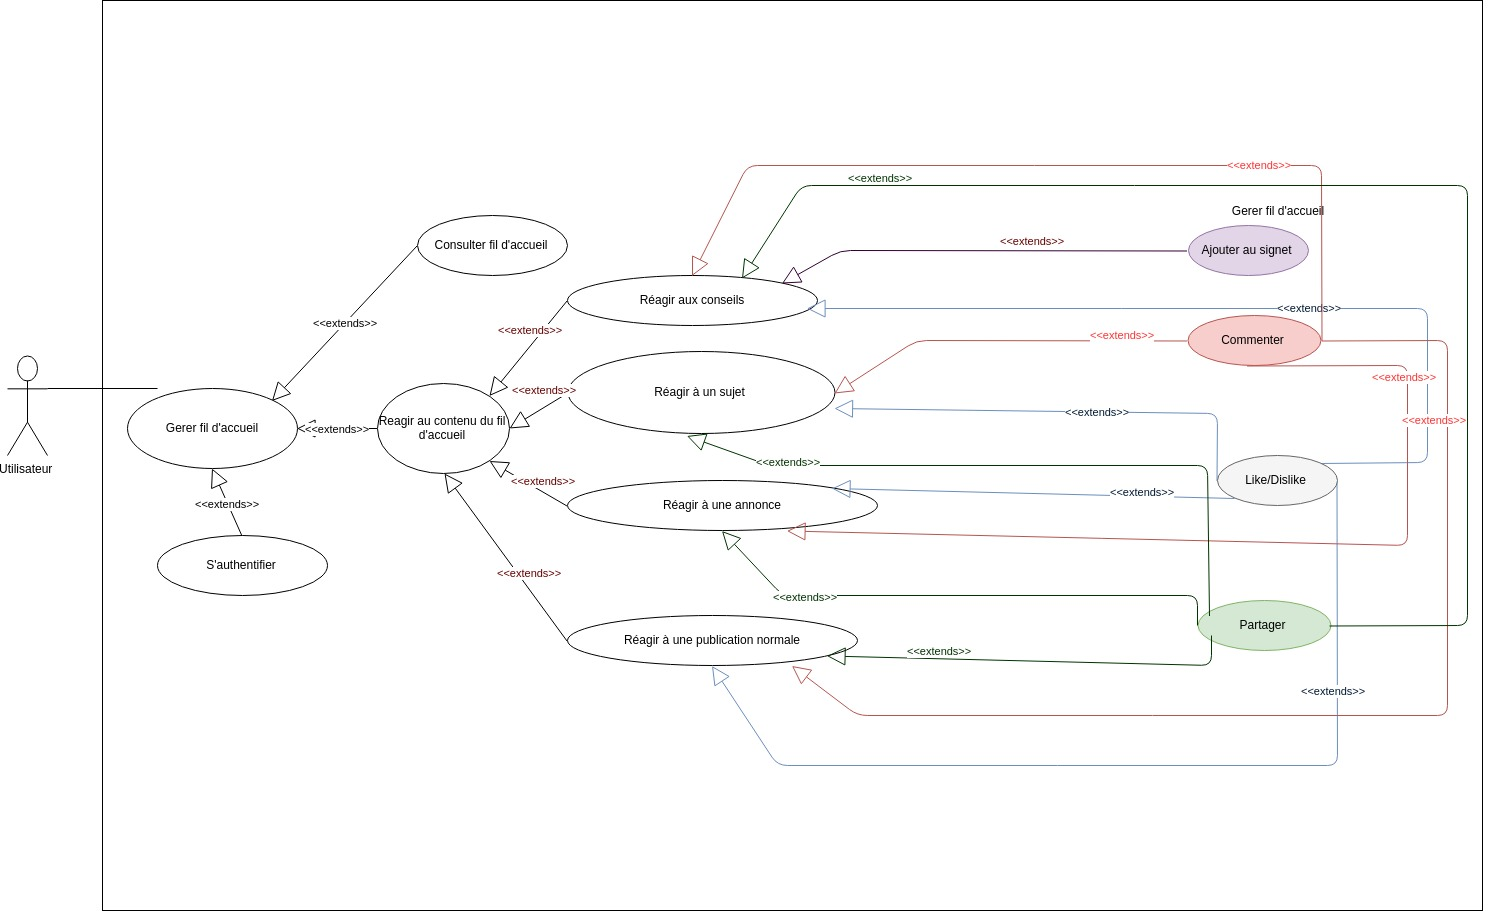
\includegraphics[width=20cm, height=16cm, angle=90]{Diagrammes/gerer_accueil}
			\caption{ Diagramme de cas d’utilisation « Gérer fil d'accueil »}
			\label{fig:gereraccueil}
		\end{figure}
		
		\begin{tabular}{ |p{3cm}|p{10cm}|  }
			
			\hline
			Titre&  Gérer il d'accueil\\
			\hline
			Description  & L’application permet aux Utilisateurs de mettre à jour leur fil d’actualité ,de réagir à des publications, de les commenter , de les partager\\
			\hline
			Acteur&Utilisateur\\
			\hline
			Pré-Condition & S'authentifier 
			\\
			\hline
			1- Consulter fil d'accueil & L’utilisateur peut consulter son fil d’accueil et visualiser les publications partagé par ses contact et les annonces à proximité ainsi que les sujet de discussion partagé par l’administrateur\\
			
			2- Reagir au contenu du fil d'accueil & 
			\begin{itemize} 
				\item Réagir au conseils
				\begin{itemize}
					\item J’aime/Je n’aime pas
					\item Commenter
					\item Partager
					\item Ajouter au signet 
				\end{itemize}
				\item Réagir à un sujet 
				\begin{itemize}
					\item J'aime / Je n'aime pas 
					\item Commenter
				\end{itemize}
				\item Réagir à une annonce
				\begin{itemize}
					\item J’aime/Je n’aime pas
					\item Commenter
					\item Partager
				\end{itemize}
				\item Réagir à une publication normale
				\begin{itemize}
					\item J’aime/Je n’aime pas
					\item Commenter
					\item Partager
				\end{itemize}
				\end {itemize} \\
				\hline
				Post-Condition& Fil d'actualité Géré\\
				\hline
				Exception& Pas d'accès Internet . \\
				\hline
			\end{tabular}
			
			\subsubsection{Cas d’utilisation : Contrôler les annonces}
			\begin{figure}[H]
				\centering
				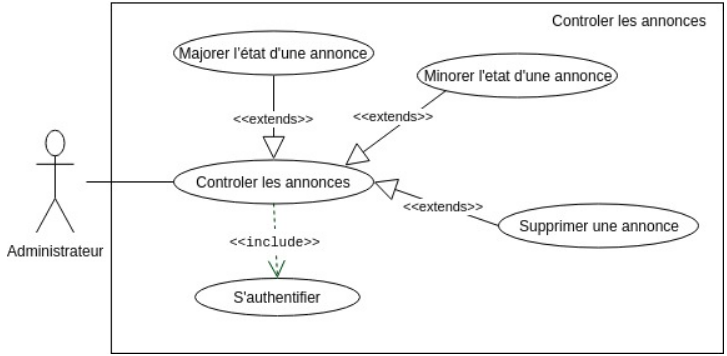
\includegraphics[width=1\textwidth]{Diagrammes/controle_annonces}
				\caption{Diagramme de cas d’utilisation « Contrôler les annonces »}
				\label{fig:controleannonces}
			\end{figure}
			
			\begin{tabular}{ |p{3cm}|p{6cm}|  }
				
				\hline
				Titre&  Contrôler les annonces\\
				\hline
				Description  & 
				L’administrateur a la possibilité de contrôler les annonces des utilisateurs\\
				\hline
				Acteur&  Administrateur .\\
				\hline
				Pré-Condition & \begin{itemize}
					\item S’authentifier.
					\item Existence de l’annonce
				\end{itemize}
				\\
				\hline
				\multicolumn{2}{|c|}{Scenario normal} \\
				\hline
				\multicolumn{2}{|c|}{L’administrateur peut consulter les annonces publié par les utilisateurs ,}\\
				%	\vspace{5mm} %5mm vertical space
				\multicolumn{2}{|c|}{	 ainsi il a la possibilité de :}\\
				\multicolumn{2}{|c|}{1- augmenter l’état d’urgence d’une annonce .} \\
				\multicolumn{2}{|c|}{2- diminuer l’état d’urgence d’une annonce .} \\
				\multicolumn{2}{|c|}{3- supprimer une annonce lorsqu’elle sont contenu est indésirable . } \\
				
				\hline
				Post-Condition& Annonce contrôlé / modifié  \\
				\hline
				Exception&  Pas d’accès internet. 
				\\
				\hline
			\end{tabular}
			\subsubsection{Cas d’utilisation : Poster sujet de discussion}
			\begin{figure}[H]
				\centering
				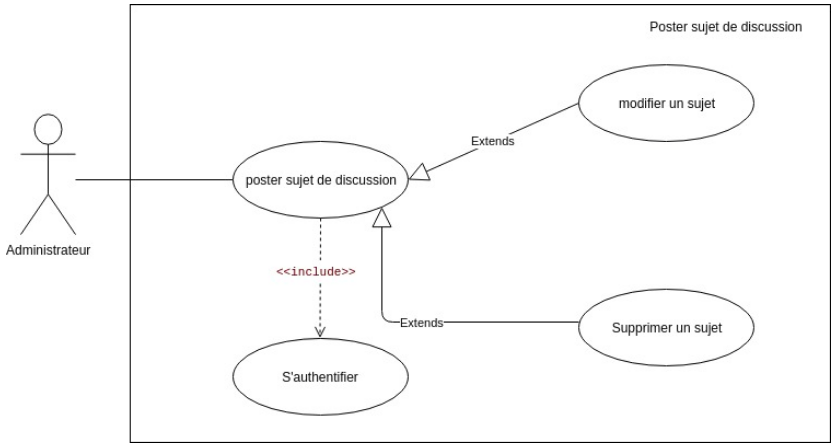
\includegraphics[width=1\textwidth]{Diagrammes/poster_sujet}
				\caption{Diagramme de cas d’utilisation «Poster sujet de discussion »}
				\label{fig:postersujet}
			\end{figure}
			
			\begin{tabular}{ |p{4cm}|p{9cm}|  }
				
				\hline
				Titre&  Poster sujet de discussion\\
				\hline
				Description  & L’administrateur de l’application peut poster un sujet de discussion .Ce poste sera visible à tout les utilisateurs ou ces dernier peuvent contribuer et partager leur avis\\
				\hline
				Acteur& 
				Administrateur
				\\
				\hline
				Pré-Condition & S’authentifier.
				\\
				\hline
				\multicolumn{2}{|c|}{Scenario normal} \\
				\hline
				
				1.Poster un sujet: &En se situant sur son espace d’administration , l’administrateur pour créer un sujet de discussion et le partager pour le rendre visible aux utilisateur \\
				2.Modifier/supprimer un sujet : & L’administrateur peut modifier le contenu du sujet ou même le supprimé \\
				% \multicolumn{2}{|c|}{2-} \\
				% \multicolumn{2}{|c|}{3- } \\
				% \multicolumn{2}{|c|}{4- } \\
				
				\hline
				Post-Condition&Sujet publié , modifié ou supprimer\\
				\hline
				Exception& 
				\begin{itemize}
					\item Pas d’accès internet.
					\item Champs vide
					\item Pas d’accès internet 
				\end{itemize}
			 \\
			 \hline
			\end{tabular}
		
			\section{Spécification préliminaire des maquettes}	
			\subsection{Front Office}
			\begin{figure}[H]
				\centering
				\includegraphics[width=1\textwidth]{Images/chp2/frontOffice}
				\caption{Maquette de l'application pour la Front Office}
				\label{fig:frontoffice}
			\end{figure}
			\begin{itemize}
				\item La première image représente  l'interface de connexion à l'application
				\item  La deuxième image représente le profil d'un utilisateur ami(e)
				\item La troisième image représente l'interface d'accueil de l'application
			\end{itemize}
			\subsection{Back Office}
			\begin{figure}[H]
				\centering
				\includegraphics[width=1\textwidth]{"newest maquettes/changement de mot de passe"}
				\caption{Gestion de profil d'un administrateur}
				\label{fig:changement-de-mot-de-passe}
			\end{figure}
			\begin{figure}[H]
				\centering
				\includegraphics[width=1\textwidth]{"newest maquettes/Screenshot from 2018-05-24 02-00-17"}
				\caption{Visualisation des listes des sujets}
				\label{fig:screenshot-from-2018-05-24-02-00-17}
			\end{figure}
			\section{Conclusion}
			Dans ce chapitre nous avons détaillé les besoins de notre application en citant les besoins fonctionnels et non fonctionnels qui sont indispensables pour mieux faciliter le travail à réaliser. Ensuite nous avons étudié les technologies les plus connus pour choisir ionic 3 pour le développement de l’application mobile , Angular 5 comme système de front end du back office et Firebase comme un système de back end de gestion et de manipulation de données. Ensuite nous avons mis en œuvre le diagramme de cas d’utilisation
			et la conception préliminaire des maquettes. Nous pouvons alors entamer la phase de conception du système.
			%%%%%%%%%%%%%%%%%%%%%%%%%%%%%%%%%%%%%%%%%%%%%%%%%%%%%%%%%%%%%%%%%%
			%                       CHAPITRE 3%                              %
			%%%%%%%%%%%%%%%%%%%%%%%%%%%%%%%%%%%%%%%%%%%%%%%%%%%%%%%%%%%%%%%%%%
			\chapter{Conception}
			\section{Introduction}
			Dans ce chapitre , nous passons à la conception qui est la phase la plus importante dans le cycle de développement d’une application pour produire une solution de haute qualité. Dans laquelle, on présentera des différents diagrammes UML.
			Pour ce faire , nous commençons par présenter l’architecture global de notre solution ce qui nous permettra de détailler nos choix conceptuels à travers les diagrammes appropriés .
			
			\section{Architecture 2-tiers Firebase}
			Définir un modèle architecturale n’est pas une tâche simple car le modèle choisi doit être compatible avec les technologies à utiliser, nous avons décidé d'adopter l’architecture 2-tiers Firebase, qui nous permettra de définir notre patron de conception : 
			\\
			
			\textbf{L’architecture 2-tiers Firebase}  ressemble beaucoup à l’architecture 3 tiers traditionnelle  ( client , serveur , base de données ) sauf que la différence est l’absence de la couche serveur . En effet , on ne peut pas dire que la couche serveur est totalement absente car le back end Firebase offre des service rendant cette architecture “Servless” d’une manière abstraite puisque les traitement sur les données de notre application s’effectue à travers des échanges “realtime “ de façon transparente entre le client (Front End) et la base de données comme indiqué sur la figure suivante :  
			\begin{figure}[H]
				\centering
				\includegraphics[width=1\textwidth]{"Images/ch4/Architecture 2-tiers Firebase"}
				\caption{L’architecture 2-tiers Firebase}
				\label{fig:architecture-2-tiers-firebase}
			\end{figure}
			\section{Architecture MVC(Modèle-vue-contrôleur)}
			Modèle-vue-contrôleur ou MVC est un motif d'architecture logicielle destiné aux interfaces graphiques . Le motif est composé de trois types de modules ayant trois responsabilités différentes : les modèles, les vues et les contrôleurs.
			\begin{itemize}
				\item \textbf{Modèle} \\ Élément qui contient les données ainsi que de la logique en rapport avec les données: validation, lecture et enregistrement . Il peut, dans sa forme la plus simple, contenir uniquement une simple valeur, ou une structure de données plus complexe.
				
				\item \textbf{Vue} \\ Partie visible d'une interface graphique. La vue se sert du modèle, et peut être un diagramme, un formulaire, des boutons, etc. Une vue contient des éléments visuels ainsi que la logique nécessaire pour afficher les données provenant du modèle.
				
				\item \textbf{Contrôleur} \\ Module qui traite les actions de l'utilisateur, modifie les données du modèle et de la vue
			\end{itemize}
			\begin{figure}[H]
				\centering
				\includegraphics[width=13cm, height=5.2cm]{"Images/ch3/Capture du 2018-05-22 19-49-45"}
				\caption{Model-View-Controller (MVC)}
				\label{fig:capture-du-2018-05-22-19-49-45}
			\end{figure}
			
			\section{Conception detaillé }
			\subsection{Vue de kruchten}
			Le modèle « 4+1 » vues, dit de Kruchten, d’un système informatique permet d’organiser la description du système en plusieurs vues complémentaires, chacune présentant le système selon un point de vue différent. L’utilisation de vues permet de traiter séparément les intérêts des divers groupes d’intervenants et ainsi de mieux séparer les préoccupations fonctionnelles et les préoccupations extra fonctionnelles .
			\begin{figure}[H]
				\centering
				\includegraphics[width=1\textwidth]{"Images/ch3/Modele_architecture_Kruchten"}
				\caption{Vue de Kruchten}
				\label{fig:400px-modelearchitecturekruchten}
			\end{figure}
			\subsubsection{Vue de cas d’utilisation}
			Un cas d’utilisation est défini comme un ensemble de scénarios d’utilisation, chaque scénario représentant une séquence d’interaction des utilisateurs (acteurs) avec le système. L’intérêt des cas d’utilisation est de piloter l’analyse par les exigences des utilisateurs. Ceux-ci se sentent concernés car ils peuvent facilement comprendre les cas d’utilisation qui les concernent. Cette méthode permet donc d’aider à formaliser les véritables besoins et attentes des utilisateurs. cette vue présente le :
			\\
			
			\textbf{• Diagramme de cas d’utilisation}
			
			\textbf{• Diagramme de package}
			\subsubsection{Vue logique}
			La vue logique constitue la principale description architecturale d’un système informatique et beaucoup de petits projets se contentent de cette seule vue. La vue logique permet d’identifier les différentes éléments et mécanismes du système à réaliser. cette vue présente le :
			\\
			
			\textbf{• Diagramme de classes}
			
			\textbf{• Diagramme d’objet}
			\subsubsection{La vue processus}
			La vue des processus décrit les interactions entre les différents processus. Cette vue permet de vérifier le respect des contraintes de fiabilité et des performances des systèmes multitâches. cette vue présente le :
			\\
			
			\textbf{• Diagramme de séquence}
			\\
			
			Les diagrammes de séquences permettent de représenter des collaborations entre objets selon un point de vue temporel, on y met l’accent sur la chronologie des envois de messages. Il permet de décrire comment les éléments du système interagissent entre eux et avec les acteurs en se basant sur deux dimensions.\\
			
			Dimension vertical (axe de temps) :l’ordre d’envoi d’un message est déterminé par sa position sur l'axe vertical du diagramme, le temps s’écoule de haut en bas de cet axe.
			Dimension horizontal (les objets et les acteurs) :l’ordre de disposition des objets sur l’axe horizontal est sans importance.\\
			
			Les éléments de base de ce diagramme sont :\\
			\begin{itemize}
				\item Les objets interagissent dans un scénario.
				\item Les différents types des messages envoyés :une description est écrite au dessus de la flèche.
				\item Représentation graphique de la ligne de vie de chaque objet.\\
			\end{itemize}
			
			
			\textbf{• Diagramme d’activité}\\
			
			C’est un Diagramme associé à un objet particulier ou à un ensemble d’objets, qui illustre les flux entre les activités et les actions. Il permet de représenter graphiquement le déroulement d’un cas d’utilisation. Composition d’un diagramme d’activités
			Le diagramme d’activité se compose des éléments suivants :
			\\
			
			\textbf{Une activité} représente une exécution d’un mécanisme , autrement dit, un déroulement
			d’étapes séquentielles.\\
			
			\textbf{Une transition} qui représente Le passage d’une activité vers une autre. Cette transition peut être automatique, qui se déclenche par la fin d’une activité, provoquent le début immédiat d’une autre ou conditionnelle ,qui ne se déclenche qu’après la satisfaction de la condition qu’on appelle aussi garde.
			\\
			
			\textbf{Les gardes} qui représentent la condition de passage d’une activité à une autre dans les transitions conditionnelles ils sont symbolisés par des losanges.
			\subsubsection{La vue de réalisation }
			La vue de réalisation permet de visualiser l’organisation des composants dans l’environnement de développement. Elle permet également de gérer la configuration.
			cette vue présente le :
			\\
			
			\textbf{• Diagramme de composants}
			\\
			
			Le diagramme de composants définit l’architecture logicielle du système dans un environnement de développement donné. Il est issu de la conception et permet de représenter le système et les sous-systèmes du modèle physique de l’architecture logicielle à réaliser. Un système ou un sous-système définit un espace de visibilité et regroupe des classes.
			\subsubsection{La vue de déploiement}
			La vue de déploiement représente le système dans son environnement d’exécution. Elle traite des contraintes géographiques (distribution des processeurs dans l’espace), des contraintes de bandes passantes, du temps de réponse et des performances du système ainsi que de la tolérance aux fautes et aux pannes. Cette vue est fort utile pour l’installation et la maintenance régulière du système. cette vue présente le :
			\\
			
			\textbf{• Diagramme de déploiement}
			\\
			
			Les diagrammes de déploiement sont utilisés pour représenter l’architecture physique d’un système. Ils montrent la distribution des composants logiciels sur la base d’unités d’exécution (les nœuds).
			\subsection{Conception de cas d’utilisation "Gérer profile"}
			\subsubsection{Vue processus :Diagramme de séquence}
			\begin{tabular}{ |p{3cm}|p{8cm}|  }
				
				\hline
				Titre& Gérer le profil \\
				\hline
				Description  & L’utilisateur a la possibilité de gérer son profil\\
				\hline
				Acteur&Utilisateur .\\
				\hline
				Pré-Condition &S’authentifier.
				\\
				\hline
				\multicolumn{2}{|c|}{Scénario normal} \\
				\hline
				1- Modifier ses informations personnelles & L’utilisateur peut modifier ses informations personnel tel que numéro de téléphone , langue , adresse ou description .\\
				
				2- Gérer ses publication & 
				\begin{itemize} 
					\item Créer conseil 
					\item Gérer contenu privée
					\item Gérer des publications normales 
					\end {itemize} \\
					3- Gérer Compte&
					\begin{itemize}
						\item Modifier mot de passe 
						\item Se déconnecter
					\end{itemize}\\
					\hline
					Post-Condition& Profil géré\\
					\hline
					Exception&  Pas d’accès internet .\\
					\hline
					
				\end{tabular}
				\captionof{table}{Description textuelle du cas d'utilisation « Gérer profile »}
				
				La figure suivante représente le diagramme de séquence <<Gérer profile>>  où l’utilisateur peut gérer son contenu privé ,son compte et ses publications et modifier ses informations personnels.
				
				\begin{figure}[H]
					\centering
					\includegraphics[width=0.85\linewidth]{"Images/ch3/sequenceGererProfil"}
					\caption{Diagramme de séquence «Gérer profile»}
					\label{fig:gestion-de-profil-complet}
				\end{figure}
				
				\subsubsection{Vue logique :Diagramme de classes}
				\begin{figure}[H]
					\centering
					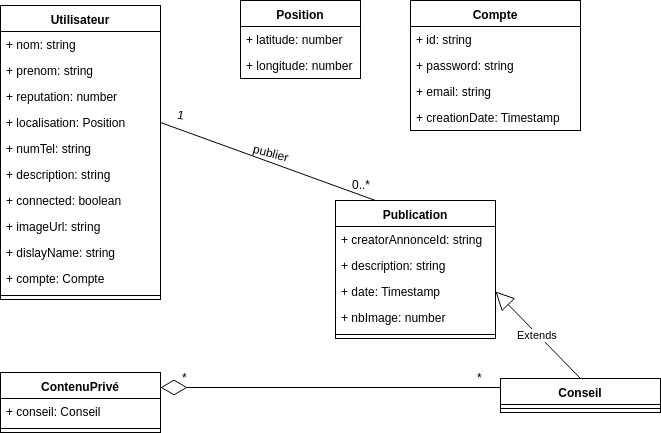
\includegraphics[width=1\textwidth]{Images/ch3/ClasseGererProfile}
					\caption{Diagramme de classes «Gérer profile»}
					\label{fig:classegererprofile}
				\end{figure}
				
				\subsubsection{Vue de réalisation :Digramme de composant}
				\begin{figure}[H]
					\centering
					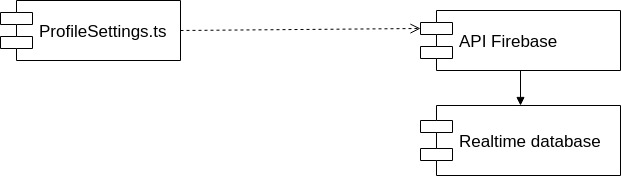
\includegraphics[width=1.2\textwidth]{Images/ch3/ComposantProfileSettings}
					\caption{Diagramme de composant «Gérer profile»}
					\label{fig:composantprofilesettings}
				\end{figure}
				
				
				\subsubsection{Vue de déploiement :Diagramme de déploiement}
				\begin{figure}[H]
					\centering
					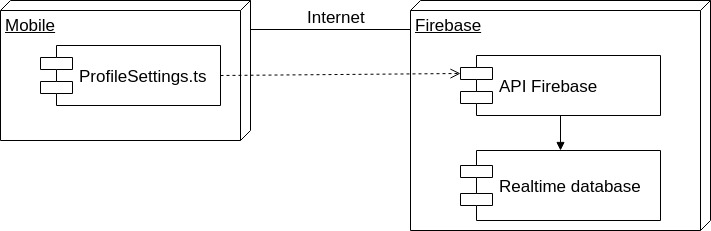
\includegraphics[width=1\textwidth]{Images/ch3/deploimentProfileSettings}
					\caption{Diagramme de déploiement «Gérer profile»}
					\label{fig:deploimentprofilesettings}
				\end{figure}
				\subsection{Conception de cas d’utilisation "Poster annonce"}
				\subsubsection{Vue processus :Diagramme de séquence}
				\begin{tabular}{ |p{3cm}|p{11cm}|  }
					
					\hline
					Titre&  Poster des annonces\\
					\hline
					Description  &L’application permet aux utilisateurs de publier des annonces d’animaux en cas d’urgences de 4 types (annonce de besoin d’aide A3, annonce de besoin de
					foyer A2, annonce de besoin d’un spécialiste A1, annonce d’un animal en danger A0).
					\\
					\hline
					Acteur&Utilisateur\\
					\hline
					Pré-Condition &Vérification de la validité de session et la réputation de l’utilisateur en cas d’une annonce du type A1 ou A0 et l’activation du GPS 
					\\
					\hline
					\multicolumn{2}{|c|}{Scenario normal} \\
					\hline
					Déclarer une annonce&L’utilisateur doit choisir le type d'annonce, puis accéder à l’interface de déclaration d’annonce où il doit introduire une description et il peut aussi ajouter des images et il précise sa localisation.
					
					
					\vspace{5mm} %5mm vertical space
					Dans le cas ou la réputation de l’utilisateur est supérieure à 30 points , il peut poster une annonce de n’importe quel type.
					
					
					\vspace{5mm} %5mm vertical space
					Dans le cas ou la réputation de l’utilisateur est inférieur à 30 points , il a le droit de poster des annonces seulement de type A3 ou A2 .
					
					
					\vspace{5mm} %5mm vertical space
					L’avantage des annonces A0 et A1 est que la notification de ces annonces atteints les utilisateurs dans une zone géographique de 8 Km pour A1 et 10 Km pour A0 .
					\\
					
					\hline
					Post-Condition& Annonce publiée\\
					\hline
					Exception&  • Exception 1 :Champs obligatoires incomplets 
					
					• Exception 2 : Désactivation du GPS
					
					
					• Exception 3 : Pas d'accès Internet .\\
					\hline
				\end{tabular}
				\captionof{table}{Description textuelle du cas d'utilisation « poster annonce »}
				\begin{figure}[H]
					\centering
					\includegraphics[width=1.15\textwidth]{"Images/ch3/_Poster Annonce"}
					\caption{Diagramme de séquence «Poster annonce»}
					\label{fig:poster-annonce}
				\end{figure}
				\subsubsection{Vue logique :Diagramme de classes}
				\begin{figure}[H]
					\centering
					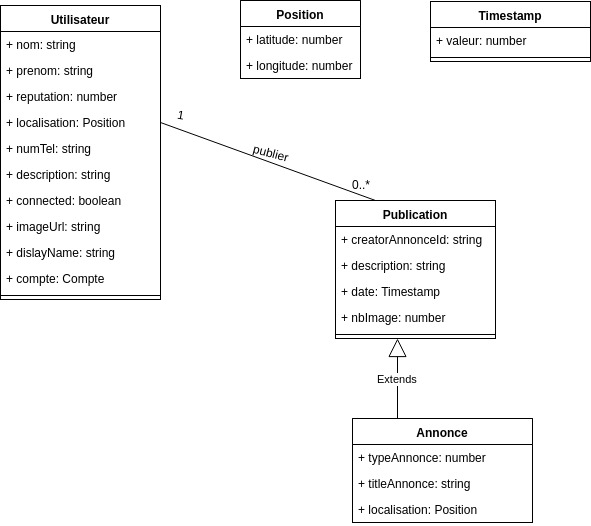
\includegraphics[width=1\textwidth]{Images/ch3/classePosterAnnonce}
					\caption{ Diagramme de classes «Poster annonce»}
					\label{fig:classeposterannonce}
				\end{figure}
				\subsubsection{Vue de réalisation :Diagramme de composant}
				\begin{figure}[H]
					\centering
					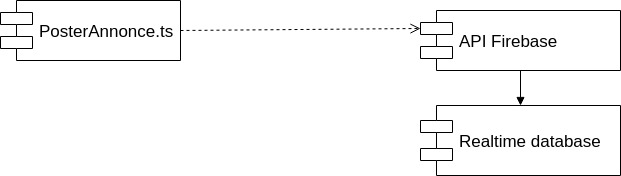
\includegraphics[width=1\textwidth]{Images/ch3/ComposantPosterAnnonce}
					\caption{Diagramme de composant «Poster annonce»}
					\label{fig:composantposterannonce}
				\end{figure}
				\subsubsection{Vue de déploiement :Diagramme de déploiement}
				\begin{figure}[H]
					\centering
					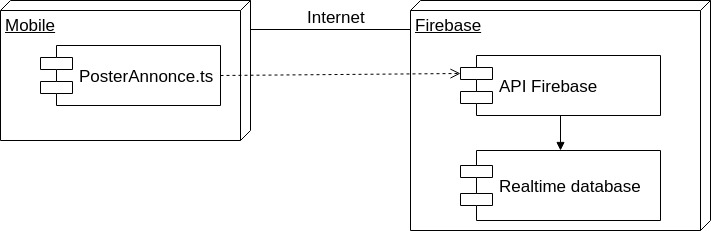
\includegraphics[width=1\textwidth]{Images/ch3/deploimentPosterAnnonce}
					\caption{Diagramme de déploiement «Poster annonce»}
					\label{fig:deploimentposterannonce}
				\end{figure}
				\subsection{Conception de cas d’utilisation "Gérer fil d'accueil"}
				\subsubsection{Vue processus :Diagramme de séquence}
				\begin{tabular}{ |p{3cm}|p{10cm}|  }
					
					\hline
					Titre&  Gérer il d'accueil\\
					\hline
					Description  & L’application permet aux Utilisateurs de mettre à jour leur fil d’actualité ,de réagir à des publications, de les commenter , de les partager\\
					\hline
					Acteur&Utilisateur\\
					\hline
					Pré-Condition & S'authentifier 
					\\
					\hline
					1- Consulter fil d'accueil & L’utilisateur peut consulter son fil d’accueil et visualiser les publications partagé par ses contact et les annonces à proximité ainsi que les sujet de discussion partagé par l’administrateur\\
					
					2- Reagir au contenu du fil d'accueil & 
					\begin{itemize} 
						\item Réagir au conseils
						\begin{itemize}
							\item J’aime/Je n’aime pas
							\item Commenter
							\item Partager
							\item Ajouter au signet 
						\end{itemize}
						\item Réagir à un sujet 
						\begin{itemize}
							\item J'aime / Je n'aime pas 
							\item Commenter
						\end{itemize}
						\item Réagir à une annonce
						\begin{itemize}
							\item J’aime/Je n’aime pas
							\item Commenter
							\item Partager
						\end{itemize}
						\item Réagir à une publication normale
						\begin{itemize}
							\item J’aime/Je n’aime pas
							\item Commenter
							\item Partager
						\end{itemize}
						\end{itemize} \\
						\hline
						Post-Condition& Fil d'actualité Géré\\
						\hline
						Exception& Pas d'accès Internet . \\
						\hline
					\end{tabular}
					\captionof{table}{Description textuelle du cas d'utilisation « Gérer fil d'accueil »}
					\begin{figure}[H]
						\centering
						\includegraphics[width=1.1\textwidth]{"Images/ch3/latestsequence"}
						\caption{Diagramme de séquence «Gérer fil d'accueil»}
						\label{fig:gestion-fil-daccueil}
					\end{figure}
				
				
				
					\subsubsection{Vue logique :Diagramme de classes}
					
					\begin{figure}[H]
						\centering
						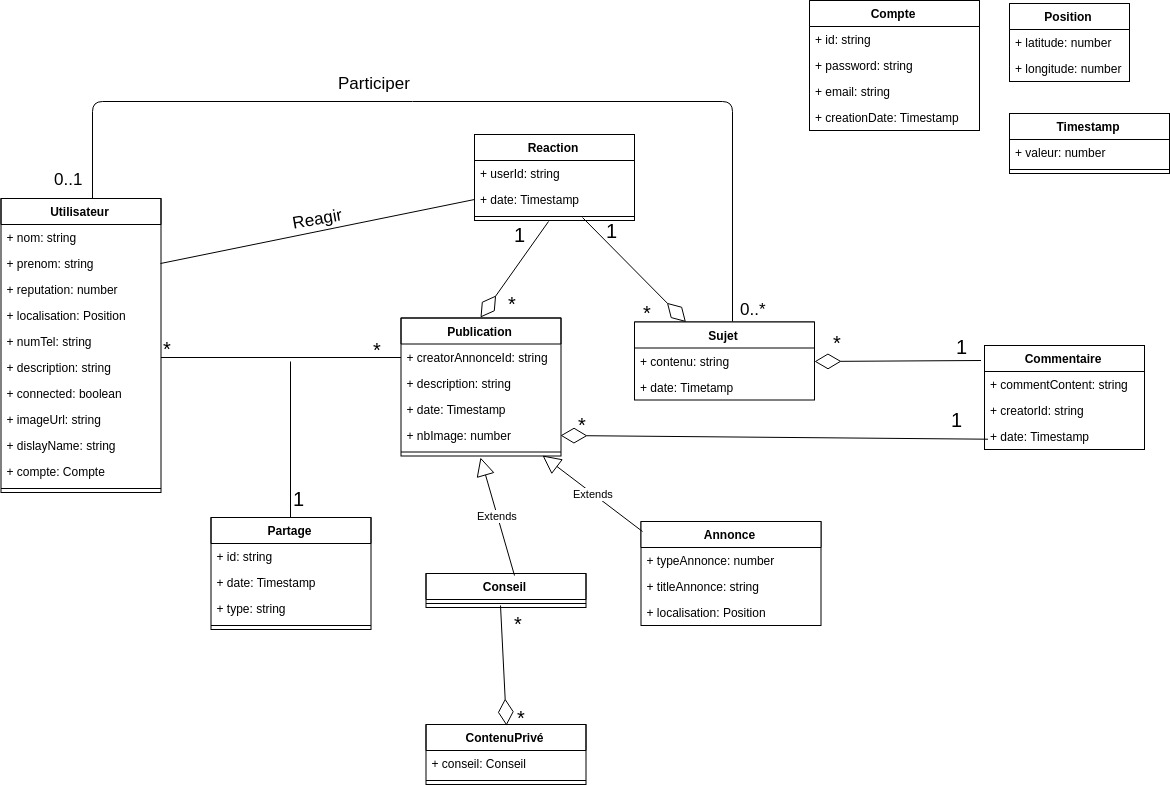
\includegraphics[width=1\textwidth]{Images/ch3/classeFilAcceuil}
						\caption{Diagramme de classes «Gérer fil d'accueil»}
						\label{fig:classefilacceuil}
					\end{figure}
					
					\subsubsection{Vue de réalisation :Diagramme de composant}
					\begin{figure}[H]
						\centering
						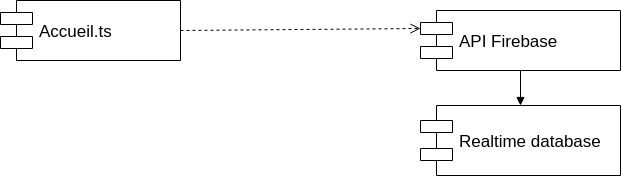
\includegraphics[width=1\textwidth]{Images/ch3/ComposantAccueil}
						\caption{Diagramme de composant «Gérer fil d'accueil»}
						\label{fig:composantaccueil}
					\end{figure}
					\subsubsection{Vue de déploiement :Diagramme de déploiement}
					\begin{figure}[H]
						\centering
						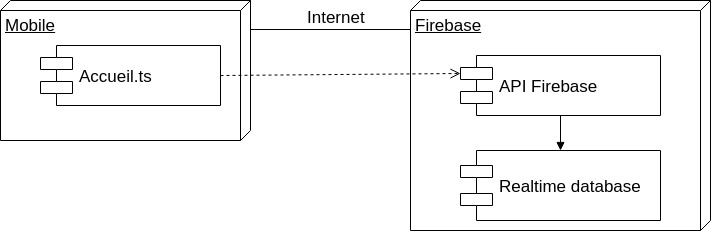
\includegraphics[width=1\textwidth]{Images/ch3/deploimentAcceuil}
						\caption{Diagramme de déploiement «Gérer fil d'accueil»}
						\label{fig:deploimentacceuil}
					\end{figure}
					\subsection{Conception de cas d’utilisation "Contrôler les annonces"}
					\subsubsection{Vue processus :Diagramme de séquence}
					\begin{tabular}{ |p{3cm}|p{6cm}|  }
						
						\hline
						Titre&  Contrôler les annonces\\
						\hline
						Description  & 
						L’administrateur a la possibilité de contrôler les annonces des utilisateurs\\
						\hline
						Acteur&  Administrateur .\\
						\hline
						Pré-Condition & \begin{itemize}
							\item S’authentifier.
							\item Existence de l’annonce
						\end{itemize}
						\\
						\hline
						\multicolumn{2}{|c|}{Scenario normal} \\
						\hline
						\multicolumn{2}{|c|}{L’administrateur peut consulter les annonces publié par les utilisateurs ,}\\
						%	\vspace{5mm} %5mm vertical space
						
						\multicolumn{2}{|c|}{ 	 ainsi il a la possibilité de :}\\
						\multicolumn{2}{|c|}{1- augmenter l’état d’urgence d’une annonce .} \\
						\multicolumn{2}{|c|}{2- diminuer l’état d’urgence d’une annonce .} \\
						\multicolumn{2}{|c|}{3- supprimer une annonce lorsqu’elle sont contenu est indésirable . } \\
						
						\hline
						Post-Condition& Annonce contrôlé / modifié  \\
						\hline
						Exception&  Pas d’accès internet. 
						\\
						\hline
					\end{tabular}
					\captionof{table}{Description textuelle du cas d'utilisation « Contrôler les annonces »}
					\begin{figure}[H]
						\centering
						\includegraphics[width=1\textwidth]{"Images/ch3/SequenceControlerAnnonce"}
						\caption{Diagramme de séquence «Contrôler les annonces»}
						\label{fig:controler-annonce}
					\end{figure}
					\subsubsection{Vue logique :Diagramme de classes}
					\begin{figure}[H]
						\centering
						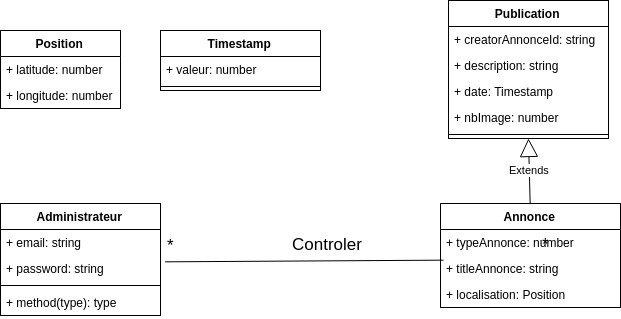
\includegraphics[width=1\textwidth]{Images/ch3/classeControlerAnnonce}
						\caption{Diagramme de classes «Contrôler les annonces»
						}
						\label{fig:classecontrolerannonce}
					\end{figure}
					
					\subsubsection{Vue de réalisation :Diagramme de composant}
					\begin{figure}[H]
						\centering
						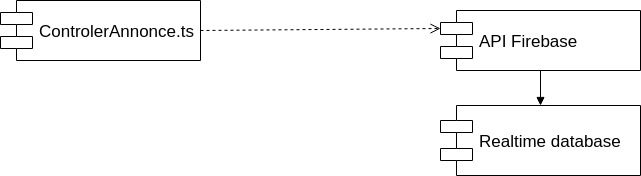
\includegraphics[width=1\textwidth]{Images/ch3/ComposantControlerAnnonce}
						\caption{Diagramme de composant «Contrôler les annonces»
						}
						\label{fig:composantcontrolerannonce}
					\end{figure}
					
					\subsubsection{Vue de déploiement :Diagramme de déploiement}
					\begin{figure}[H]
						\centering
						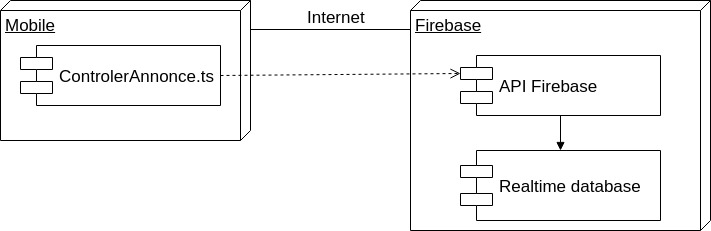
\includegraphics[width=1\textwidth]{Images/ch3/deploimentControleAnnonce}
						\caption{Diagramme de déploiement «Contrôler les annonces»
						}
						\label{fig:deploimentcontroleannonce}
					\end{figure}
				\vfill
				\vspace{30cm}
					\subsection{Diagramme de classes globale}
					Nous présentons ici le diagramme de classes globales où nous montrons les différentes classes de notre solution ainsi que les relations entre ces classes.
					\begin{figure}[H]
						\centering
						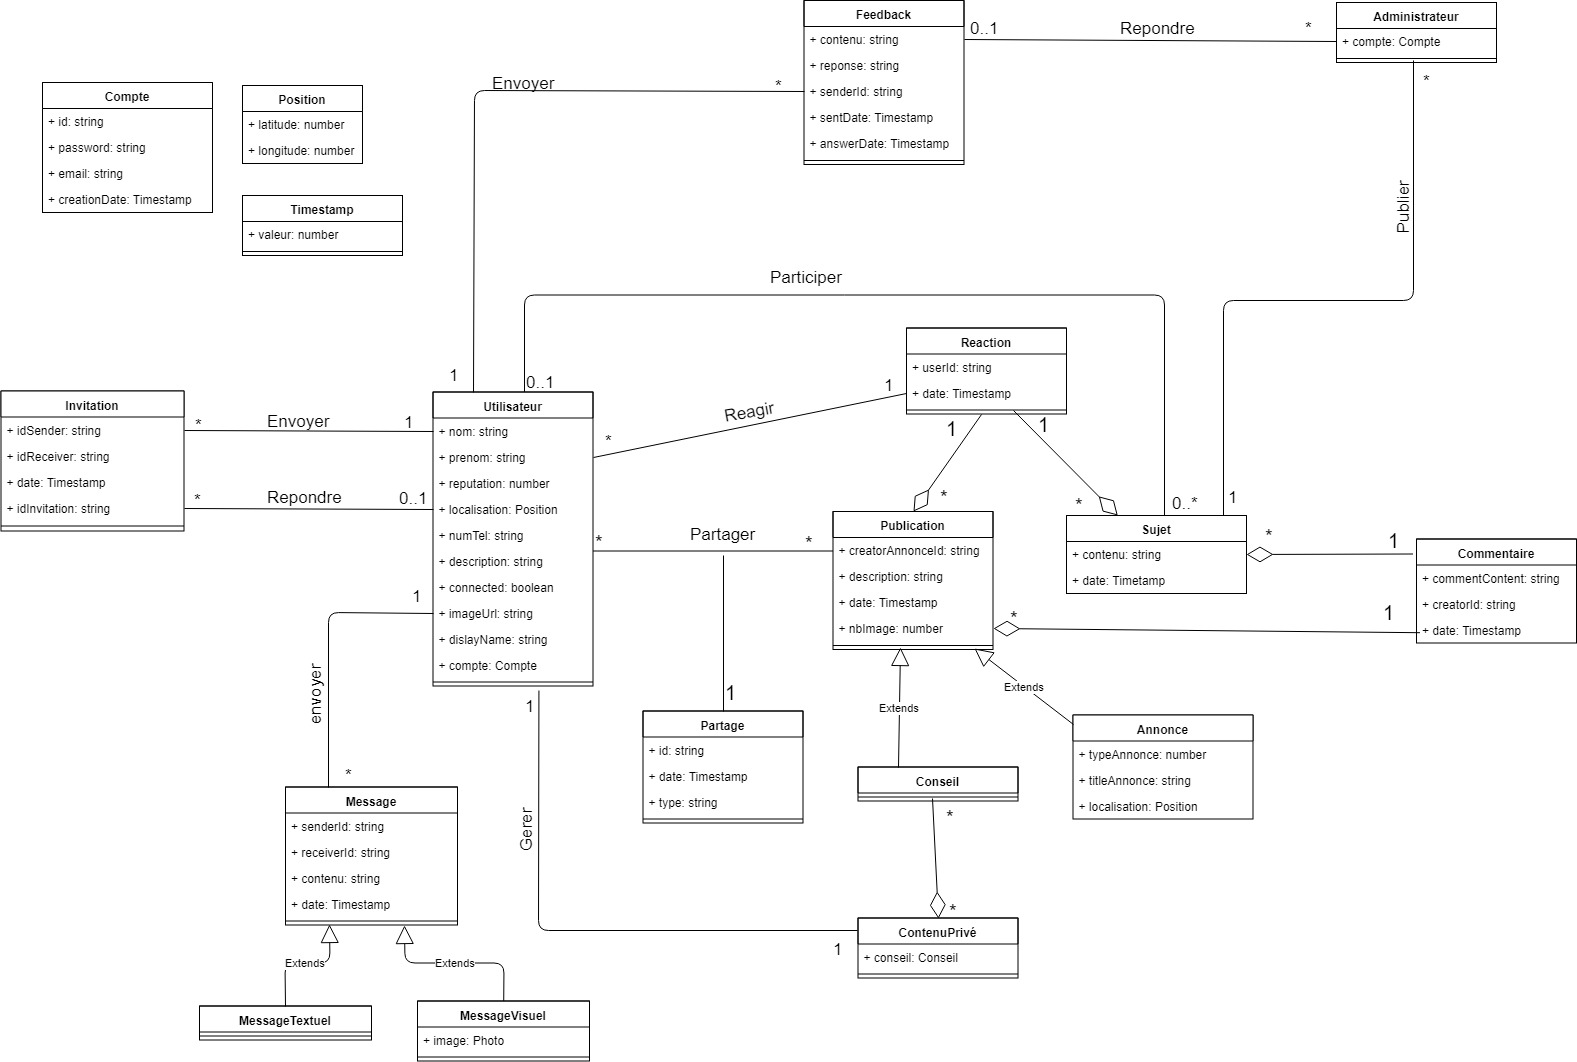
\includegraphics[width=16cm, height=15cm]{Images/ch3/classeGlobale1}
						\caption{Diagramme de classes globale}
						\label{fig:classeglobale}
					\end{figure}
				\vfill
					\section{Modèle MVC proposé}
					La figure ci dessous est un schéma simplifié de notre application qui montre la façon d’utilisation du modèle de conception MVC.
					\begin{figure}[H]
						\centering
						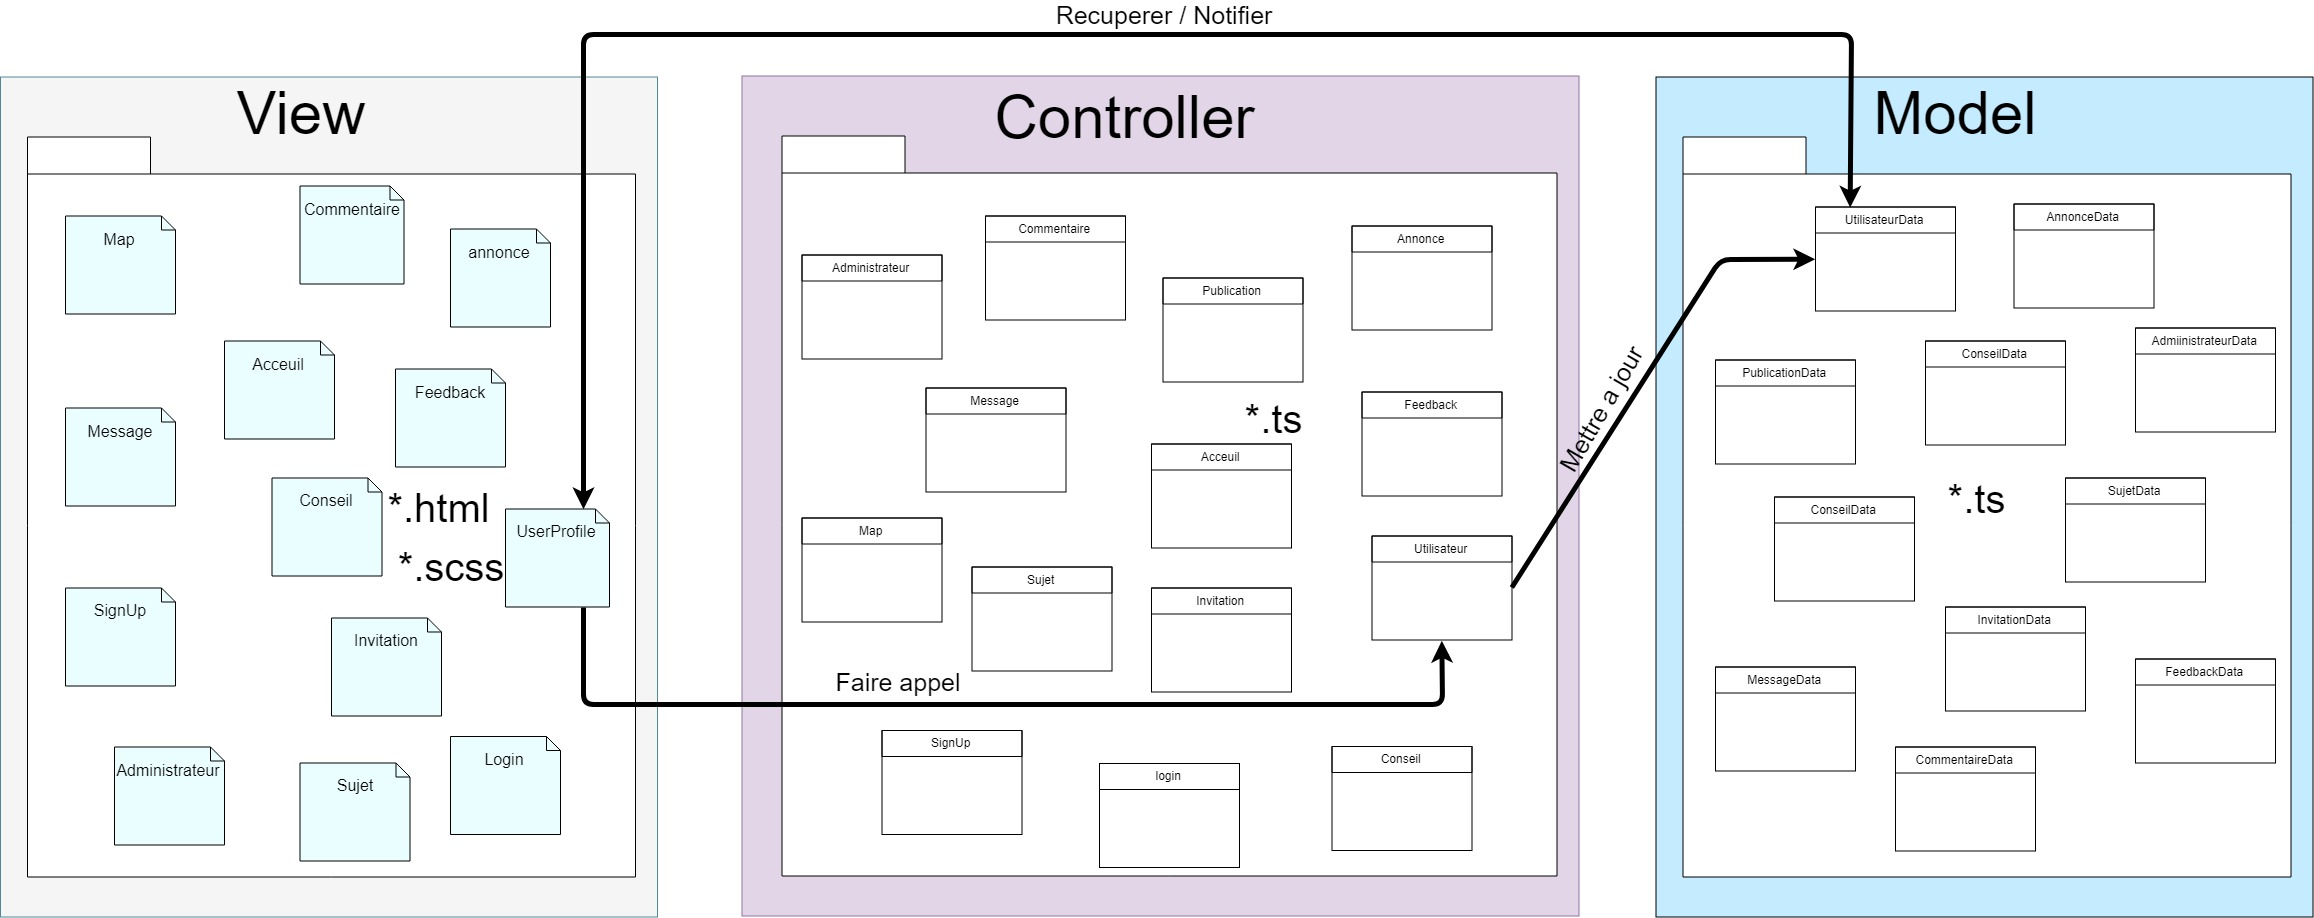
\includegraphics[width=17.5cm, height=13cm , angle=90]{Images/ch3/mvcClasseGlobal}
						\caption{Modèle MVC proposé }
						\label{fig:mvchanimo}
					\end{figure}
					
					
					\section{Conclusion}
					Dans ce chapitre nous avons présenté le modèle architecturale qu’on a adopté qui est l’architecture 2-tiers Firebase , puis l’architecture conceptuel qui est MVC . Ensuite nous avons étudié les vue de Kruchten pour réaliser la conception détaillée et enfin le diagramme de classes global.
					%%%%%%%%%%%%%%%%%%%%%%%%%%%%%%%%%%%%%%%%%%%%%%%%%%%%%%%%%%%%%%%%%%
					%                       CHAPITRE 4%                              %
					%%%%%%%%%%%%%%%%%%%%%%%%%%%%%%%%%%%%%%%%%%%%%%%%%%%%%%%%%%%%%%%%%%
					\chapter{Réalisation}
					\section{Introduction}
					La phase de réalisation est considérée comme la mise en œuvre concrète des éléments planifiés dans la recherche et déploiement de solutions pour satisfaire les objectifs définis.
					\section{Environnement de développement}
					\subsection{NodeJS}
					Node.js est une plateforme de développement Javascript avec des bibliothèques permet d'utiliser le langage JavaScript sur le serveur en dehors du navigateur.
					Node.js a été créé par Ryan Dahl dans le but de pouvoir créer des applications temps réel où le serveur est capable de pousser de l'information au client. C'est dans ce but qu'il utilise la bibliothèque libuv pour réaliser son modèle d'entrée sortie non bloquante.\\
					Pourquoi utiliser Node.js ?\\
					Node.js peut être comparé à Python, Ruby, Java, PHP. Node.js offre un environnement côté serveur et présente de nombreux intérêts:
					\begin{itemize}
						\item Logiciel libre (licence MIT)
						\item Performance du moteur v8 (un outil open source créé par Google qui analyse et exécute du code JavaScript très rapidement).
						\item Modèle non bloquant.
						\item Communauté très active.
						\item Système de paquet intégré (NPM).
						\item Les grandes entreprises l'utilisent.
					\end{itemize}
					\begin{figure}[H]
						\centering
						
\includegraphics[width=0.5\textwidth]{Images/ch4/nodejs}
						\caption{Logo NodeJs}
						\label{fig:nodejs}
					\end{figure}
					\subsection{Ionic 3 Framework}
					Ionic Framework est  un Open Source puissant SDK HTML5 permettant de développer des applications mobiles hybrides, native ou web mobile rapidement et facilement en langage WEB (HTML / CSS / JS). Il s’appuie sur AngularJS pour la partie application web du framework et sur Cordova  pour la partie construction des applications natives déployable sur plusieurs environnements tout en gardant la même interaction et design qu'une application native.
					\begin{figure}[H]
						\centering
						
\includegraphics[width=0.6\textwidth]{Images/ch4/ionic}
						\caption{Logo Ionic}
						\label{fig:ionic}
					\end{figure}
					
					\subsection{Angular 5}
					Angular est un framework JavaScript qui étend le HTML pour le rendre dynamique, et permet de développer ses propres balises et attributs HTML. C’est un framework qui se veut extensible et qui pousse vers un développement structuré, en couches, le but n’étant pas d’ajouter de simples animations au DOM, mais bien d’apporter un aspect applicatif au front-office.\\
					Les concepts qui caractérisent le plus Angular sont :
					\begin{itemize}
						\item Basé sur la logique MVC. (modèle vue contrôleur)
						\item Data-binding bidirectionnel (liaison entre vues,  contrôleurs et le modèle)
						\item Injection de dépendance (charger certaines parties de l’application seulement quand c’est nécessaire)
						\item Routing
					\end{itemize}
					\begin{figure}[H]
						\centering
						
\includegraphics[width=0.6\textwidth]{Images/ch4/angular}
						\caption{Logo Angular}
						\label{fig:angularjs}
					\end{figure}
					
					\subsection{Firebase}
					Une plateforme mobile de Google nous libère de la complexité de création et de la maintenance d’une architecture serveur performant, tout en nous garantissant une scalabilité à toute épreuve (plusieurs milliards d’utilisateurs) et une simplicité dans l’utilisation. Firebase offre plusieurs service permettant la gestion du back-end entier d’un projet.
					\begin{figure}[H]
						\centering
						
\includegraphics[width=0.7\textwidth]{Images/ch4/firebase}
						\caption{Logo Firebase}
						\label{fig:firebase}
					\end{figure}
					\subsubsection{Authentification}
					Ce service de Firebase offre les fonctionnalités de gestion des comptes des utilisateurs.
					Il permet une variété de méthode d’authentification, en utilisant un email et mot de passe , avec Facebook , avec Google plus , Twitter et bien plus.
					Après l’authentification , ce service offre les méthodes nécessaires de gestion d’un compte tel que le changement de mot de passe, la récupération de compte, vérification de la validité de session ,la connexion et la déconnexion .
						
\begin{figure}[H]
	\centering
	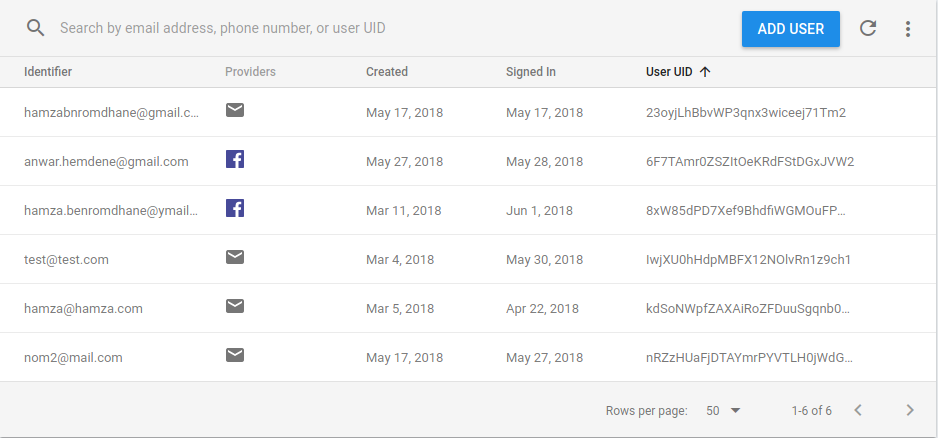
\includegraphics[width=1.3\linewidth]{Images/ch4/auth}
	\caption{Firebase authentication}
	\label{fig:auth}
\end{figure}
					\subsubsection{RealTime Database}
					Firebase Realtime Database est un service de base données NoSql permettant le stockage de données en ligne sous format JSON . Indépendamment de la plateforme, ces données sont synchronisé en temps réel pour tout client connecté. En NoSql les données sont stockés sous forme de collection d’objets et chaque objet peut contenir d’autre objet . La structuration de données est très flexible de façon que les objets d’une même collection peuvent avoir des attributs différents .
					La figure ci dessous montre une capture de notre base de données .
					
\begin{figure}[H]
	\centering
	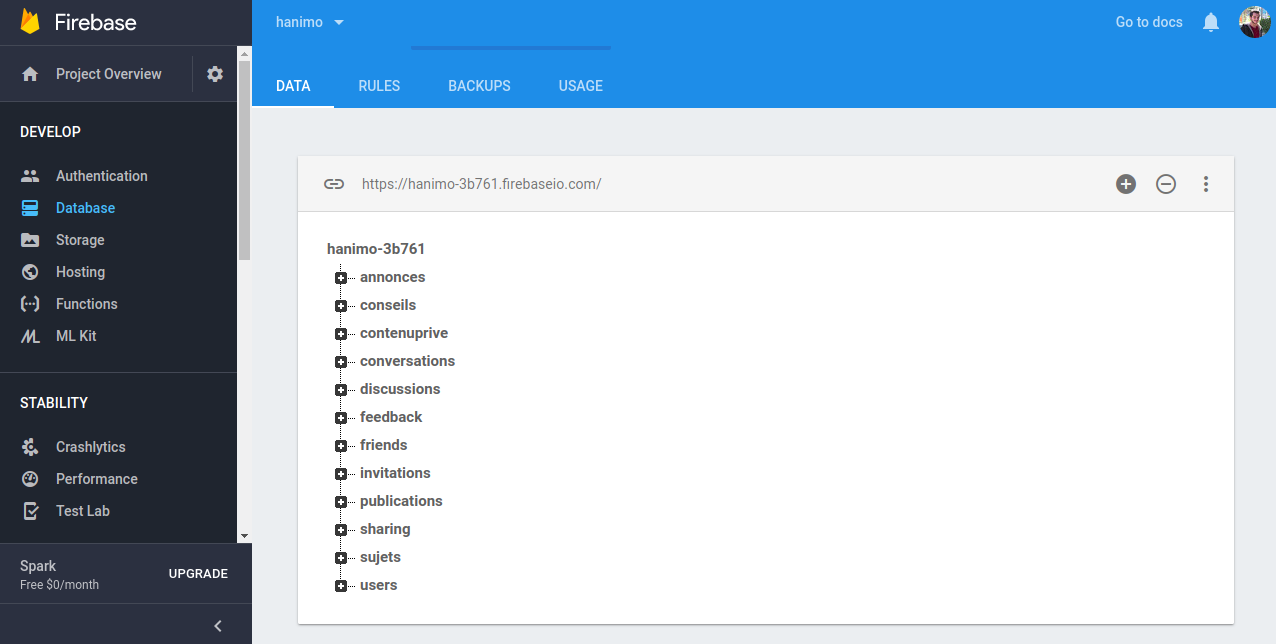
\includegraphics[width=1.3\linewidth]{Images/ch4/bd}
	\caption{Firebase Realtime Database}
	\label{fig:bd}
\end{figure}
					\subsubsection{Firebase Cloud Storage}
					
					C’est un puissant service de stockage d’objets en ligne. Il permet de stocker des images , vidéos , sons et tout type de fichier. 
					Ce service offre des méthodes pour exporter les fichiers médias du client et les stocker dans le serveur ainsi que la récupération pour les visualiser plus tard .
					
					La figure suivante présente la structuration de stockage des données média de notre application. 
					
					
					
\begin{figure}[H]
	\centering
	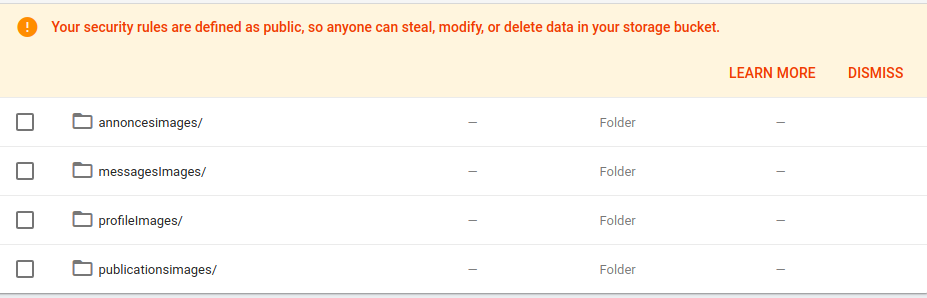
\includegraphics[width=1.3\linewidth]{Images/ch4/storage}
	\caption{Firebase Cloud Storage}
	\label{fig:storage}
\end{figure}
					
					
					

					
					\subsection{Draw.io}
					Draw.io est une application gratuite en ligne qui permet de dessiner des diagrammes ou des organigrammes. Cet outil nous propose de concevoir toutes sortes de diagrammes et les exporter sous plusieurs formats.
					\begin{figure}[H]
						\centering
						\includegraphics[width=0.6\textwidth]{Images/ch4/drawio}
						\caption{Logo Draw.io}
						\label{fig:draw}
					\end{figure}
					\subsection{Github}
					Le nom GitHub est composé du mot « git » faisant référence au système de contrôle de version open-source et le mot « hub » faisant référence au réseau social bâti autour du système Git.
					\textbf{Git} un logiciel de gestion de version, ce qui signifie qu’il gère les modifications d’un projet sans en écraser toutes les parties.
					\begin{figure}[H]
						\centering
						\includegraphics[width=1\linewidth]{Images/ch4/github}
						\caption{Page d'accueil de Github}
						\label{fig:github}
					\end{figure}
					\subsection{Inkscape}
					Inkscape est un puissant éditeur libre d'images vectorielles, sous licence GNU/GPL. Il permet la création et la manipulation de graphismes en format SVG avec des fonctionnalités similaires à celles de logiciels propriétaires du secteur tels que Illustrator, CorelDraw, Freehand, Xara Xtreme etc.
					\begin{figure}[H]
						\centering
						\includegraphics[width=1\linewidth]{Images/ch4/inkscape}
						\caption{Page d'accueil de Inkscape}
						\label{fig:github}
					\end{figure}
					\subsection{Visual Studio Code}
					Visual Studio Code est un éditeur de code open-source, gratuit et multi-plateforme, développé par Microsoft.Principalement conçu pour le développement d'application avec JavaScript, TypeScript et Node.js, l'éditeur peut s'adapter à d'autres types de langages grâce à un système d'extension bien fourni.
					\begin{figure}[H]
						\centering
						\includegraphics[width=0.7\linewidth]{Images/ch4/vsc}
						\caption{Logo Visual Studio Code}
						\label{fig:vsc}
					\end{figure}
					
					\section{Présentation de la solution "Hanimo"}
					\subsection{Front Office}
					\subsubsection{Interface de connexion }
					C’est la première interface qui s’affiche, à partir de laquelle l’utilisateur peut se connecter à son compte soit en entrant ses coordonnées , adresse mail et mot de passe, soit en se connectant avec son compte Facebook ou Gmail . Ou il peut créer un compte en appuyant sur le bouton “ créer un compte ”.
					\begin{figure}[H]
						\centering
						\includegraphics[width=0.6\textwidth]{../Maquettes/Hanimo-maquettes/Output/01-Login-Page-filled}
						\caption{Interface de connexion}
						\label{fig:01-login-page-filled}
					\end{figure}
					\subsubsection{Interface d'inscription}
					Cette interface offre à la possibilité de créer un compte sur notre application, l’utilisateur doit saisir ses informations personnels et respecter les champs qui sont obligatoires puis valider son inscription .
					\begin{figure}[H]
						\centering
						\includegraphics[width=0.7\textwidth]{../Maquettes/Hanimo-maquettes/Output/02-SignUp-Page-empty}
						\caption{Interface d'inscription}
						\label{fig:02-signup-page-empty}
					\end{figure}
\vfill

					\subsubsection{Interface de profil de l'utilisateur connecté}
					Cette interface présente le profil de l’utilisateur courant. A partir de cette interface il peut accéder au paramètre de son profil pour les modifier , changer sa photo de profil en appuyant sur l'icône de  la caméra et visualiser ses activités .
					\begin{figure}[H]
						\centering
						\includegraphics[width=0.7\textwidth]{Images/ch4/profil}
						\caption{Visualisation de profil de l'utilisateur connecté}
						\label{fig:04-my-profil-my-activity}
					\end{figure}
			\vfill
			
					\subsubsection{Interface de paramètres}
					Cette interface permet à l’utilisateur de modifier les paramètres de son compte , changer le mot de passe et choisir ses préférences de notifications
					\begin{figure}[H]
						\centering
						\includegraphics[width=0.5\textwidth]{../Maquettes/Hanimo-maquettes/Output/05-My-profile-settings-state-1}
						\caption{Interface des paramètres }
						\label{fig:05-my-profile-settings-state-1}
					\end{figure}
				\vfill
				
					\subsubsection{Interface de profil d'un ami(e)}
					Cette interface présente le profil d’un ami où on peut visualiser ses activités , ses annonces et ses publications . L’utilisateur courant peut supprimer cet ami(e) de sa liste ou lui envoyer un message privé .
					\begin{figure}[H]
						\centering
						\includegraphics[width=0.7\textwidth]{Images/ch4/friend}
						\caption{Visualisation de profil d'un ami(e)}
						\label{fig:05-view-friend-profile}
					\end{figure}\vfill\
					\subsubsection{Interface d'envoi d'une demande d'ajout en amis}
					Lorsque l’utilisateur courant accède au profil d’un autre non ami , les activités de ce dernier ne sont pas visible , donc il doit lui envoyer une invitation pour l’ajouter à sa liste d’amis comme le montre la figure suivante .
					\begin{figure}[H]
						\centering
						\includegraphics[width=0.7\textwidth]{../Maquettes/Hanimo-maquettes/Output/05-View-User-Friend-Request}
						\caption{Envoyer une demande d'ajout en amis }
						\label{fig:05-view-user-friend-request}
					\end{figure}
				\vfill
				
					\subsubsection{Interface d’annulation de l’envoi d’une demande d’ajout en amis}
					Après l’envoi d’une invitation , l'utilisateur peut changer d’avis et annuler sa demande .
					
					\begin{figure}[H]
						\centering
						\includegraphics[width=0.7\textwidth]{../Maquettes/Hanimo-maquettes/Output/05-View-User-Cancel-Friend-Request}
						\caption{Annulation de l’envoi d’une demande d’ajout en amis}
						\label{fig:05-view-user-cancel-friend-request}
					\end{figure}
				\vfill
				
					\subsubsection{Interface de profil d'un utilisateur non ami}
					Cette interface présente le profil d'un autre utilisateur non ami(e) avec l'utilisateur courant.
					\begin{figure}[H]
						\centering
						\includegraphics[width=0.7\textwidth]{../Maquettes/Hanimo-maquettes/Output/05-View-User-No-Friend}
						\caption{Profil d'un utilisateur non ami}
						\label{fig:05-view-user-no-friend}
					\end{figure}
				\vfill
				
					\subsubsection{Interface de rédaction d’un message}
					Cette interface permet de rédiger un message et l’envoyer un ami a partir de l’interface de son profil
					\begin{figure}[H]
						\centering
						\includegraphics[width=0.7\textwidth]{../Maquettes/Hanimo-maquettes/Output/05-View-User-Profile-Compose-Message}
						\caption{Composer un message}
						\label{fig:05-view-user-profile-compose-message}
					\end{figure}
				\vfill
				
					\subsubsection{Interface de fil d'accueil}
					Cette interface présente l’interface d'accueil de l’application où l’utilisateur courant peut visualiser les publication des ses amis et les annonces à proximité. Il peut ainsi commenter , aimer ou partager ces publication .
					\begin{figure}[H]
						\centering
						\includegraphics[width=0.7\textwidth]{Images/ch4/home}
						\caption{Interface de fil d'accueil}
						\label{fig:06-home-feed-with-fab}
					\end{figure}
				\vfill
				
					\subsubsection{Interface d’ajout d’annonces / publication}
					A partir de l’interface d'accueil et en appuyant sur le bouton en bas à droit l’utilisateur peut choisir le type de publication/annonce qu’il souhaite publier
					\begin{figure}[H]
						\centering
						\includegraphics[width=0.7\textwidth]{Images/ch4/home1}
						\caption{Choix de publication de divers types d'annonces}
						\label{fig:06-home-feed-with-fab-expanded}
					\end{figure}
				\vfill
				
					\subsection{Back Office}
					\subsubsection{Interface de connexion}
					Cette interface permet à l’administrateur de se connecter en introduisant son email et son mot de passe .
					\begin{figure}[H]
						\centering
						\includegraphics[width=1\textwidth]{"newest maquettes/Phase de connexion"}
						\caption{Interface de connexion}
						\label{fig:phase-de-connexion}
					\end{figure}
					\subsubsection{Interface de changement de mot de passe}
					A partir de cette interface , l’administrateur peut mettre à jour son mot de passe 
					\begin{figure}[H]
						\centering
						\includegraphics[width=1\textwidth]{"newest maquettes/changement de mot de passe"}
						\caption{Interface de gestion de profil}
						\label{fig:changement-de-mot-de-passe}
					\end{figure}
					\subsubsection{Interface d'ajout d'un nouveau sujet}
					Cette interface permet à l’administrateur de publier un nouveau sujet de discussion en remplissant les champs vide et il peut ajouter une image .
					\begin{figure}[H]
						\centering
						\includegraphics[width=1\textwidth]{"newest maquettes/ajouter sujet"}
						\caption{Interface pour ajouter un nouveau sujet}
						\label{fig:ajouter-sujet}
					\end{figure}
					\subsubsection{Interface des listes des sujets publiés }
					A partir de cette interface , l’administrateur peut visualiser les sujet publié précédemment et les commenter .
					\begin{figure}[H]
						\centering
						\includegraphics[width=1\textwidth]{"newest maquettes/Screenshot from 2018-05-24 02-00-17"}
						\caption{Interface des listes des sujets}
						\label{fig:screenshot-from-2018-05-24-02-00-17}
					\end{figure}
					\subsubsection{Interface des feedbacks}
					Cette interface présente les feedback envoyé par les utilisateurs où l’administrateur peut répondre à ces feedback .
					\begin{figure}[H]
						\centering
						\includegraphics[width=1\textwidth]{"newest maquettes/repondre au feedback"}
						\caption{Interface des feedbacks}
						\label{fig:repondre-au-feedback}
					\end{figure}
					
					\section{Conclusion}
					Dans ce chapitre nous avons présenté l’environenement logiciel utilisé lors du projet, suivi par des captures d’écran montrant les interfaces en cours de fonctionnement de notre application mobile et site web.
					\backmatter
					\chapter{Conclusion générale}
					Ce travail s’inscrit dans le cadre du projet de fin d’études en vue de l’obtention du diplôme de la
					Licence appliquée en informatique : Systèmes Informatiques et Logiciels. Il a pour objectif de développer une plateforme permettant de venir en aide à des animaux en cas de danger. \\
					
					Nous résumons ainsi le travail effectué au cours de notre projet. Nous avons mis en place un réseau social dédié aux activistes animaliers. Ce réseau va leur permettre de poster des annonces à propos d’animaux en besoins d’aide ou intervention, partager des expériences en publiant des conseils, échanger des messages privés, personnaliser leurs profils, former un réseau d’amis . Notre application est accompagnée par un back office qui est une partie administrative permettant aux administrateurs d’effectuer des tâches de contrôles tel que la modification de l'état d’urgence d’une annonce, répondre aux feedback et partager des sujets de discussion .\\
					
					Ce projet était une occasion pour apprendre de nouvelles technologies avancées. Comment réagir dans les situations de blocage et la pression de temps , respecter la spécification et surtout mieux gérer notre temps .\\
					
					Nous estimons que nous avons pu atteindre la plupart des objectifs fixés. Cependant quelque fonctionnalités reste manquantes comme l’appel vidéo et audio ainsi qu’un manque au niveau du design vu la limite du temps et la taille du projet .
					\begin{thebibliography}{9}
	\bibitem{2TUP} 
	Definition 2TUP :\
	\\\texttt{http://www.catchu.fr/accelerateur/la-demarche-projet-2tup/}
	
	\bibitem{Avantages et inconvénient développement android :} 
	Avantages et inconvénient développement android :
	\\\texttt{	https://franceyou.wordpress.com/2013/01/05/avantages-et-inconvenients-de-
		developpement-dapplications-android}
	
	\bibitem{UML} 
	Definition UML
	\\\texttt{https://www.math-info.univ-paris5.fr/ bouzy/Doc/UML-NotesCours.pdf}
	
	\bibitem{2 tiers} 
	Architecture 2 tiers image
	\\\texttt{https://www.linkedin.com/pulse/develop-2-tier-web-applications-firebase-mar
		ian-veteanu}
	
	\bibitem{diagramme de classes} 
	Definition diagramme de classe
	\\\texttt{https://www.supinfo.com/articles/single/3224-uml-diagramme-classe}
	
	\bibitem{MVC} 
	MVC
	\\\texttt{https://www.tutorialspoint.com/mvc_framework/mvc_framework_introduction.htm}
	
	\bibitem{Vue de Kruchten} 
	Vue de Kruchten
	\\\texttt{	https://docs.google.com/document/d/1PoB8jQ216G6iZHtcaku5cb5HFh
		PSJmPdlFnRtqVnbeA/edit}
	
	
	\bibitem{Github} 
	Github - présentation
	\\\texttt{http://simplonline.co/13-ressources/11-github-presentation}
	
	\bibitem{Inkscape} 
	Inkscape
	\\\texttt{https://inkscape.org/en/}
	
	\bibitem{LaTeX} 
	Introduction à LaTeX
	\\\texttt{https://www.plpeeters.com/blog/fr/post/110-introduction-a-latex}
	
	\bibitem{Environnement de développement.} 
	Environnement de développement
	\\\texttt{https://www.blog-nouvelles-technologies.fr/3461/quest-ce-quun-environnement
		-de-developpement/}
	
	\bibitem{Firebase } 
	Firebase 
	\\\texttt{https://openclassrooms.com/courses/creez-un-backend-scalable-et-performant
		-sur-firebase/titre-de-votre-premier-chapitre-222}
	
	\bibitem{Draw.io} 
	Draw.io
	\\\texttt{https://www.tice-education.fr/index.php/tous-les-articles-er-ressources/
		articles-internet/819-draw-io-un-outil-pour-dessiner-des-diagrammes-en-ligne}
	
	\bibitem{Angular} 
	Angular
	\\\texttt{http://creersonsiteweb.net/page-angular-js-angularjs-apprendre-javascript
		-cours-tuto-exemple-example}
	
	\bibitem{Ionic} 
	Ionic
	\\\texttt{https://www.supinfo.com/articles/single/155-presentation-framework-ionic}
	
	\bibitem{Nodejs} 
	Nodejs
	\\\texttt{https://makina-corpus.com/blog/metier/2014/introduction-a-nodejs}
	
	\bibitem{GANTT} 
	GANTT
	\\\texttt{http://www.gantt.com/fr/}
	
\end{thebibliography}
				\end{document} 